\chapter{Experimentation \& Results}

\pagebreak

\section{Screenshots}

\subsection{Website}

\noindent
Below are some screenshots of the website, which is hosted on the cloud. It is a Progressive Web App (PWA), meaning it can function as a functioning native Android/iOS application or a desktop web application on the same code.

\vspace*{\fill}
\begin{figure}[H]
    \centering
    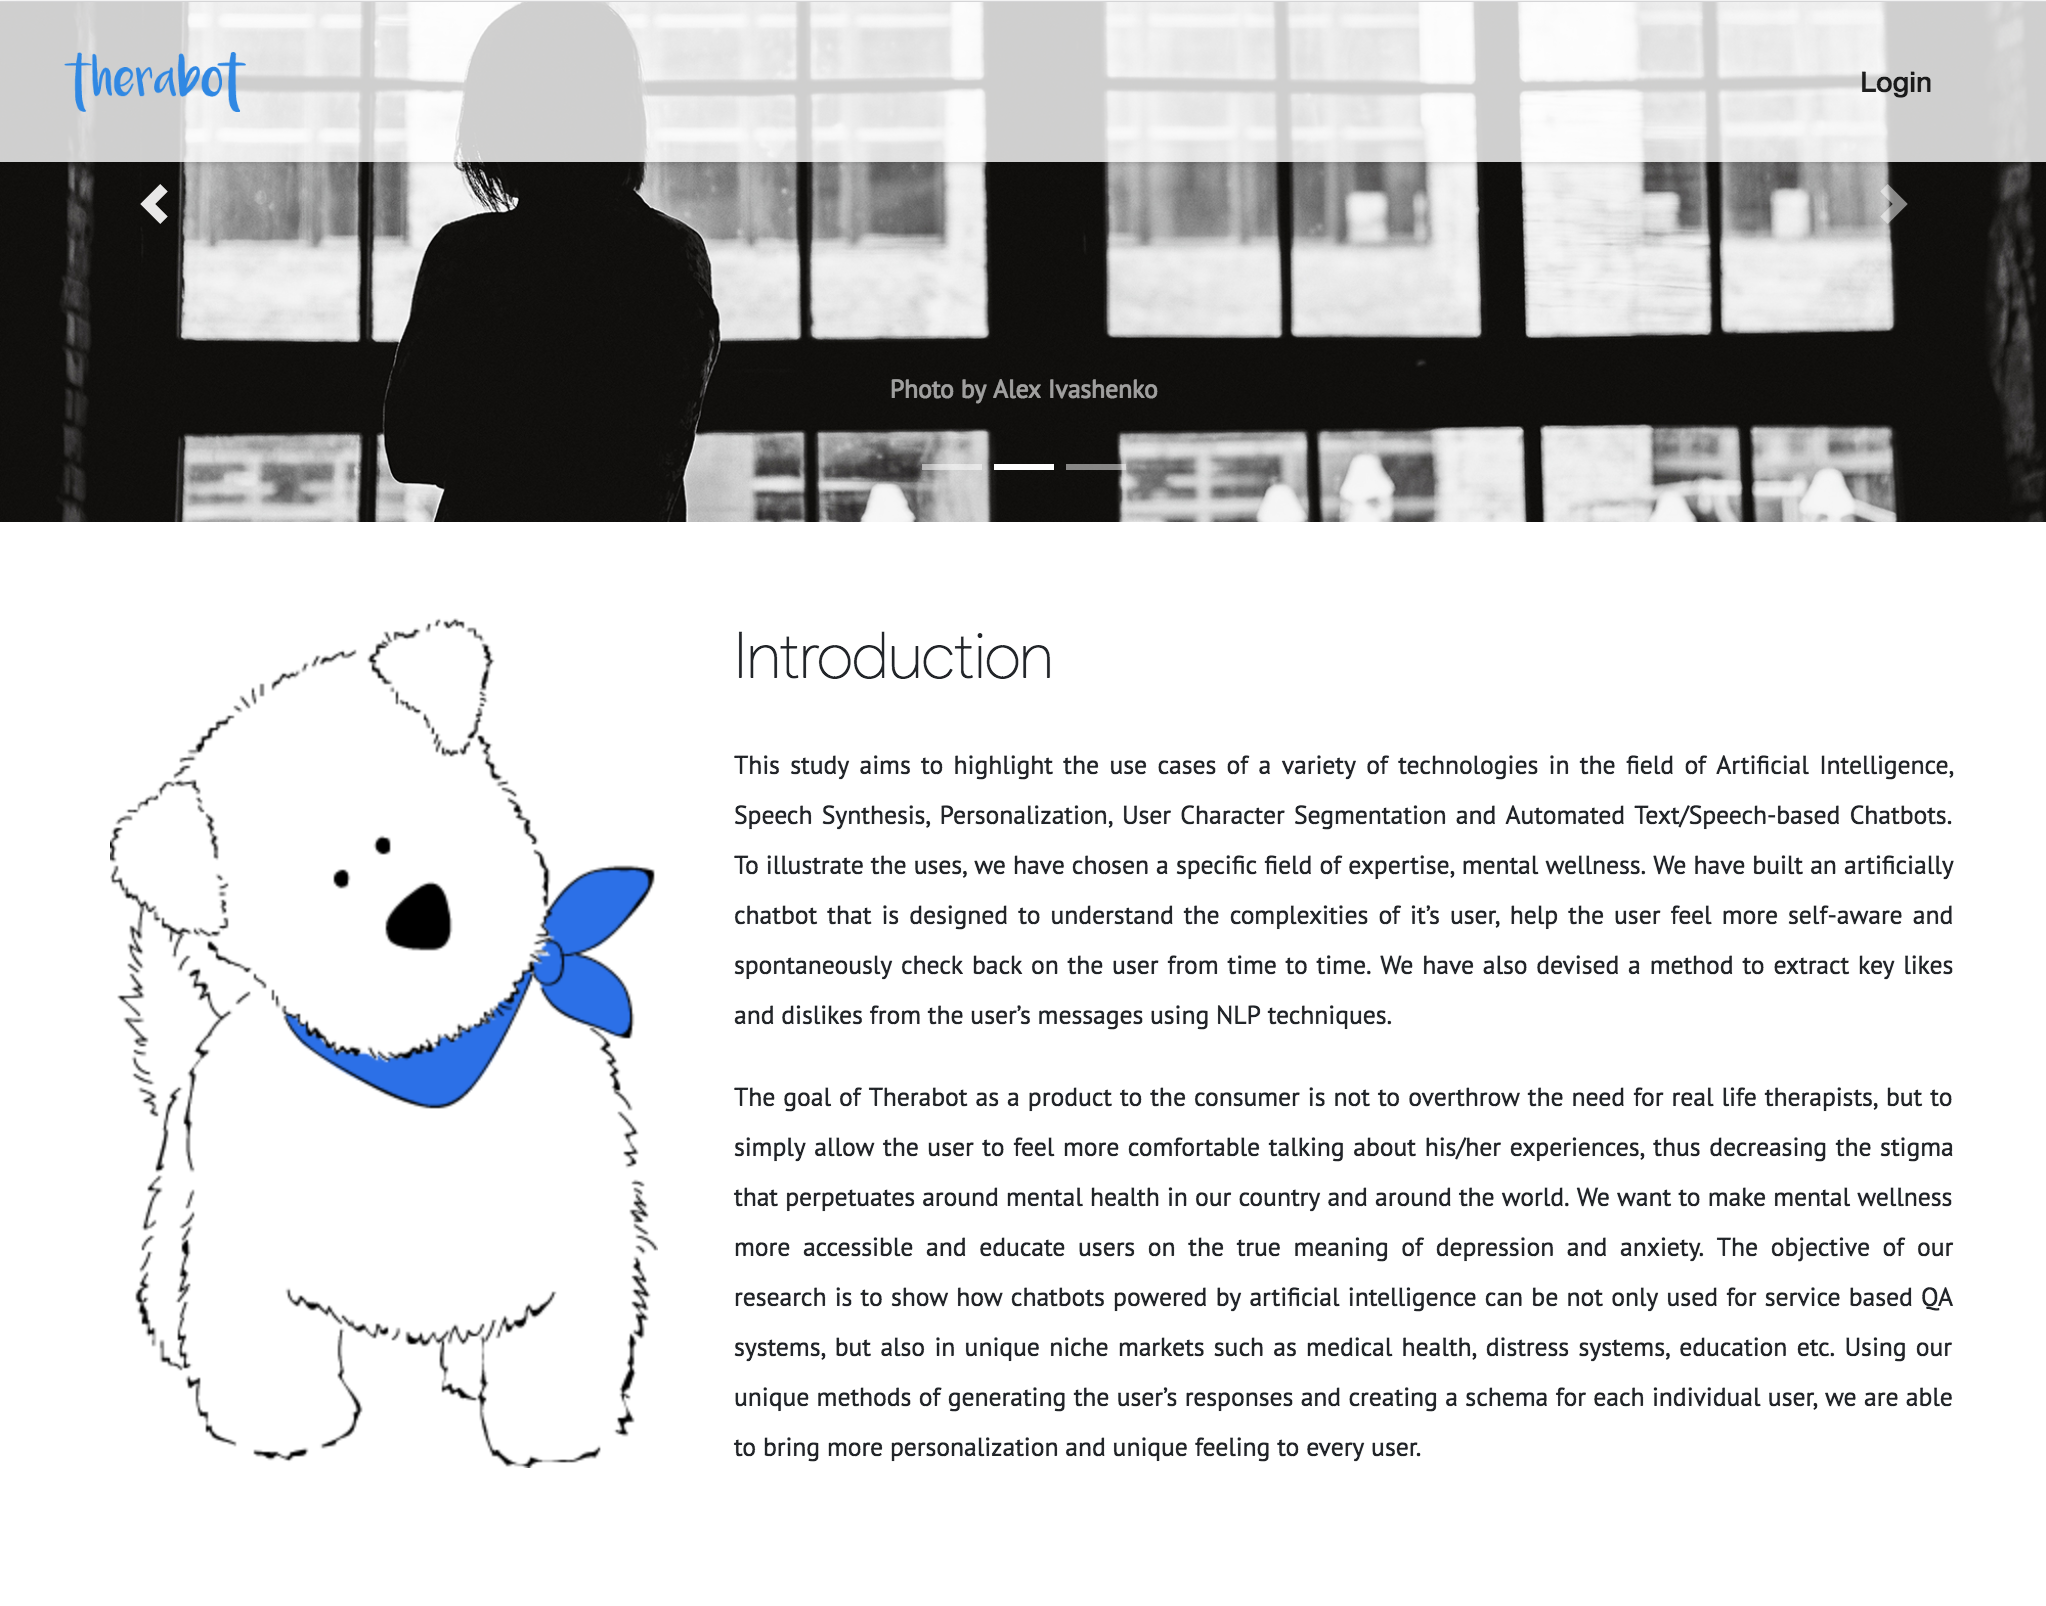
\includegraphics[width=\linewidth]{images/screenshots/website/website-introduction.png}
    \caption{Introduction}
\end{figure}
\vspace*{\fill}

\pagebreak

\vspace*{\fill}
\begin{figure}[H]
    \centering
    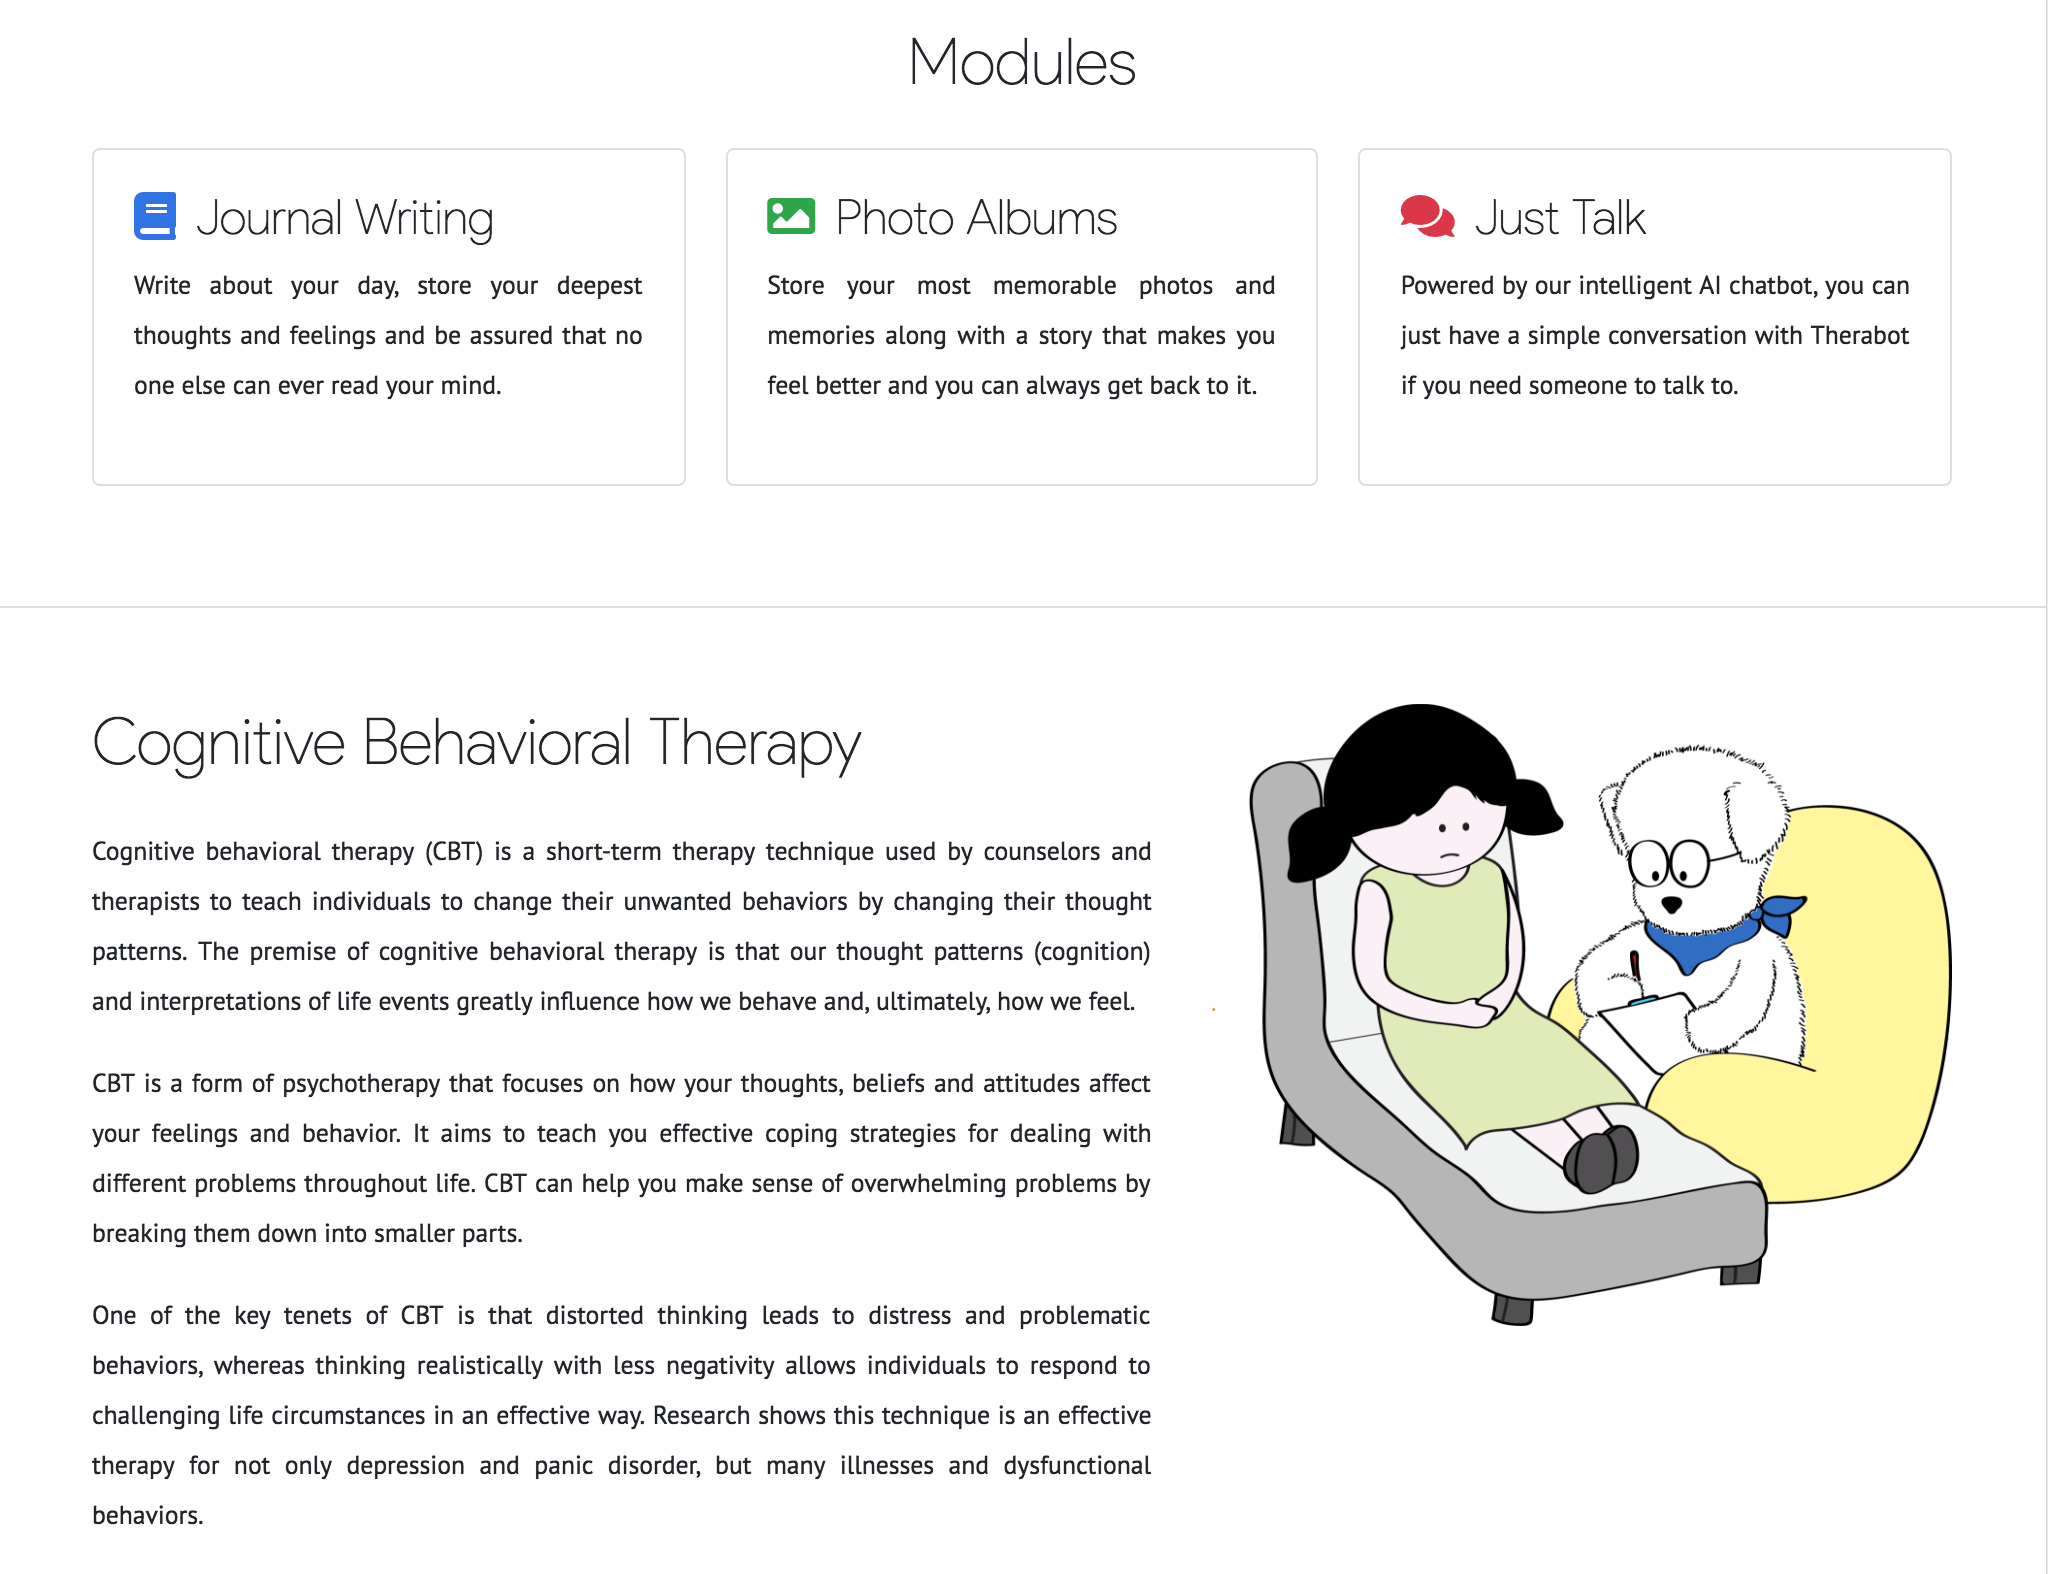
\includegraphics[width=\textwidth]{images/screenshots/website/website-cbt.png}
    \caption{Cognitive Behavioral Therapy}
\end{figure}

\begin{figure}[H]
    \centering
    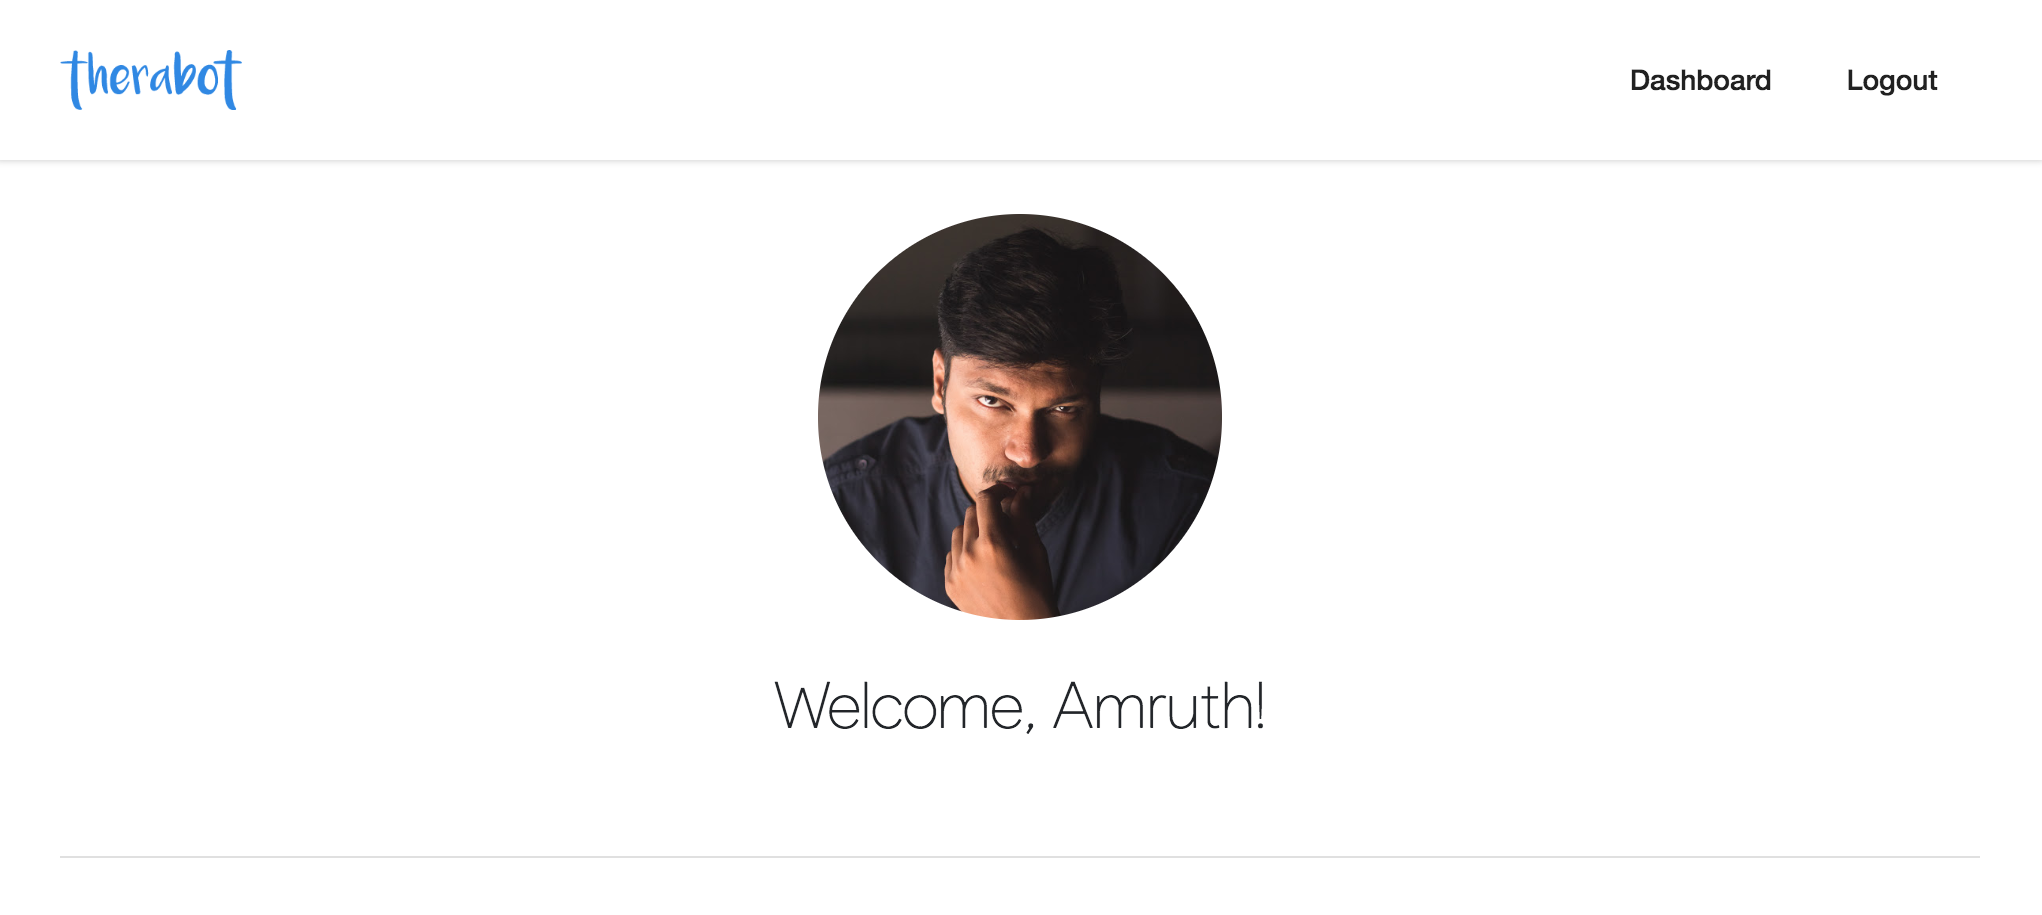
\includegraphics[width=\textwidth]{images/screenshots/website/website-welcome.png}
    \caption{Welcome - User Dashboard}
\end{figure}
\vspace*{\fill}

\pagebreak

\vspace*{\fill}
\begin{figure}[H]
    \centering
    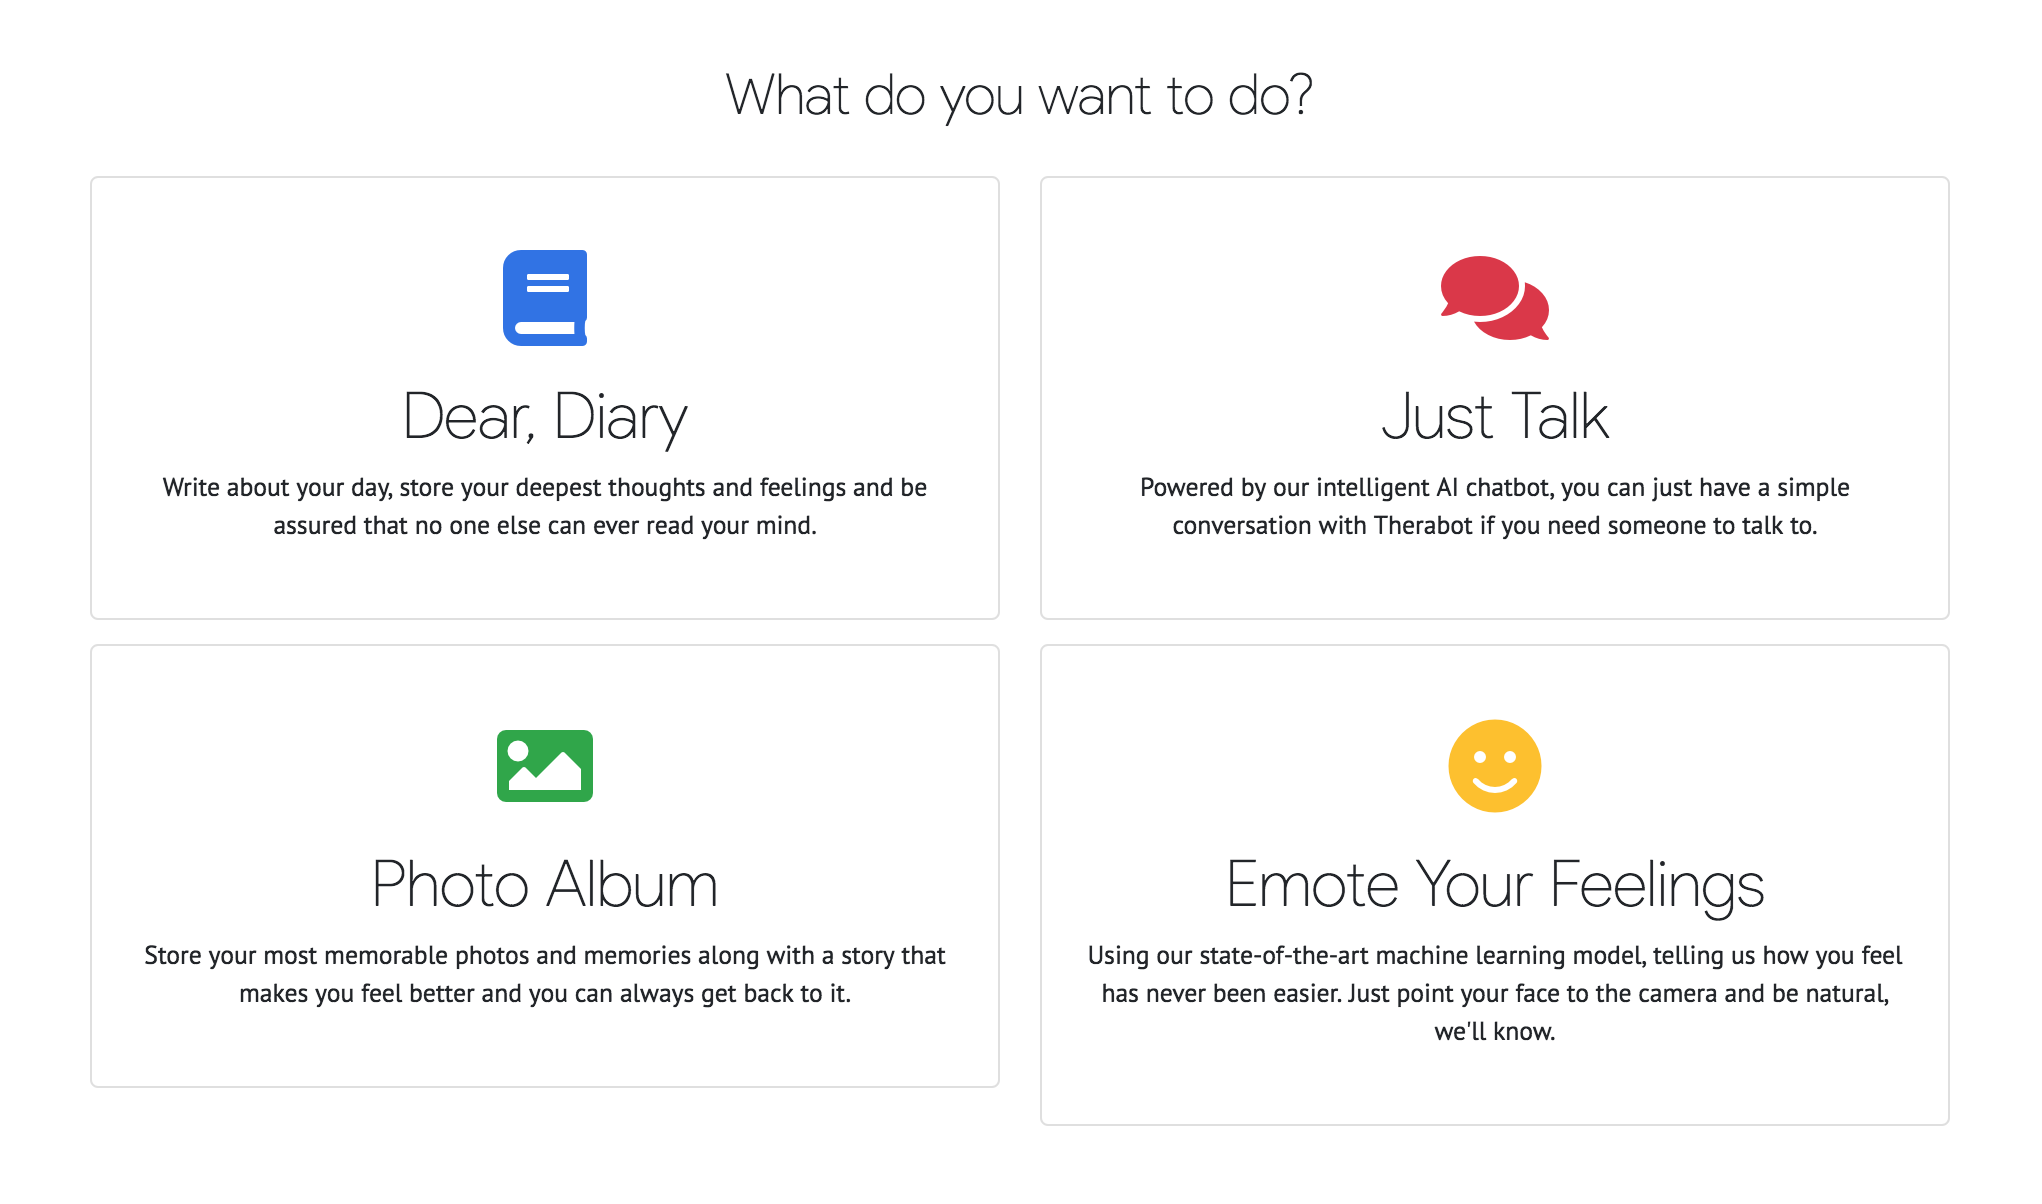
\includegraphics[width=\textwidth]{images/screenshots/website/website-modules.png}
    \caption{Modules on the Website}
\end{figure}

\begin{figure}[H]
    \centering
    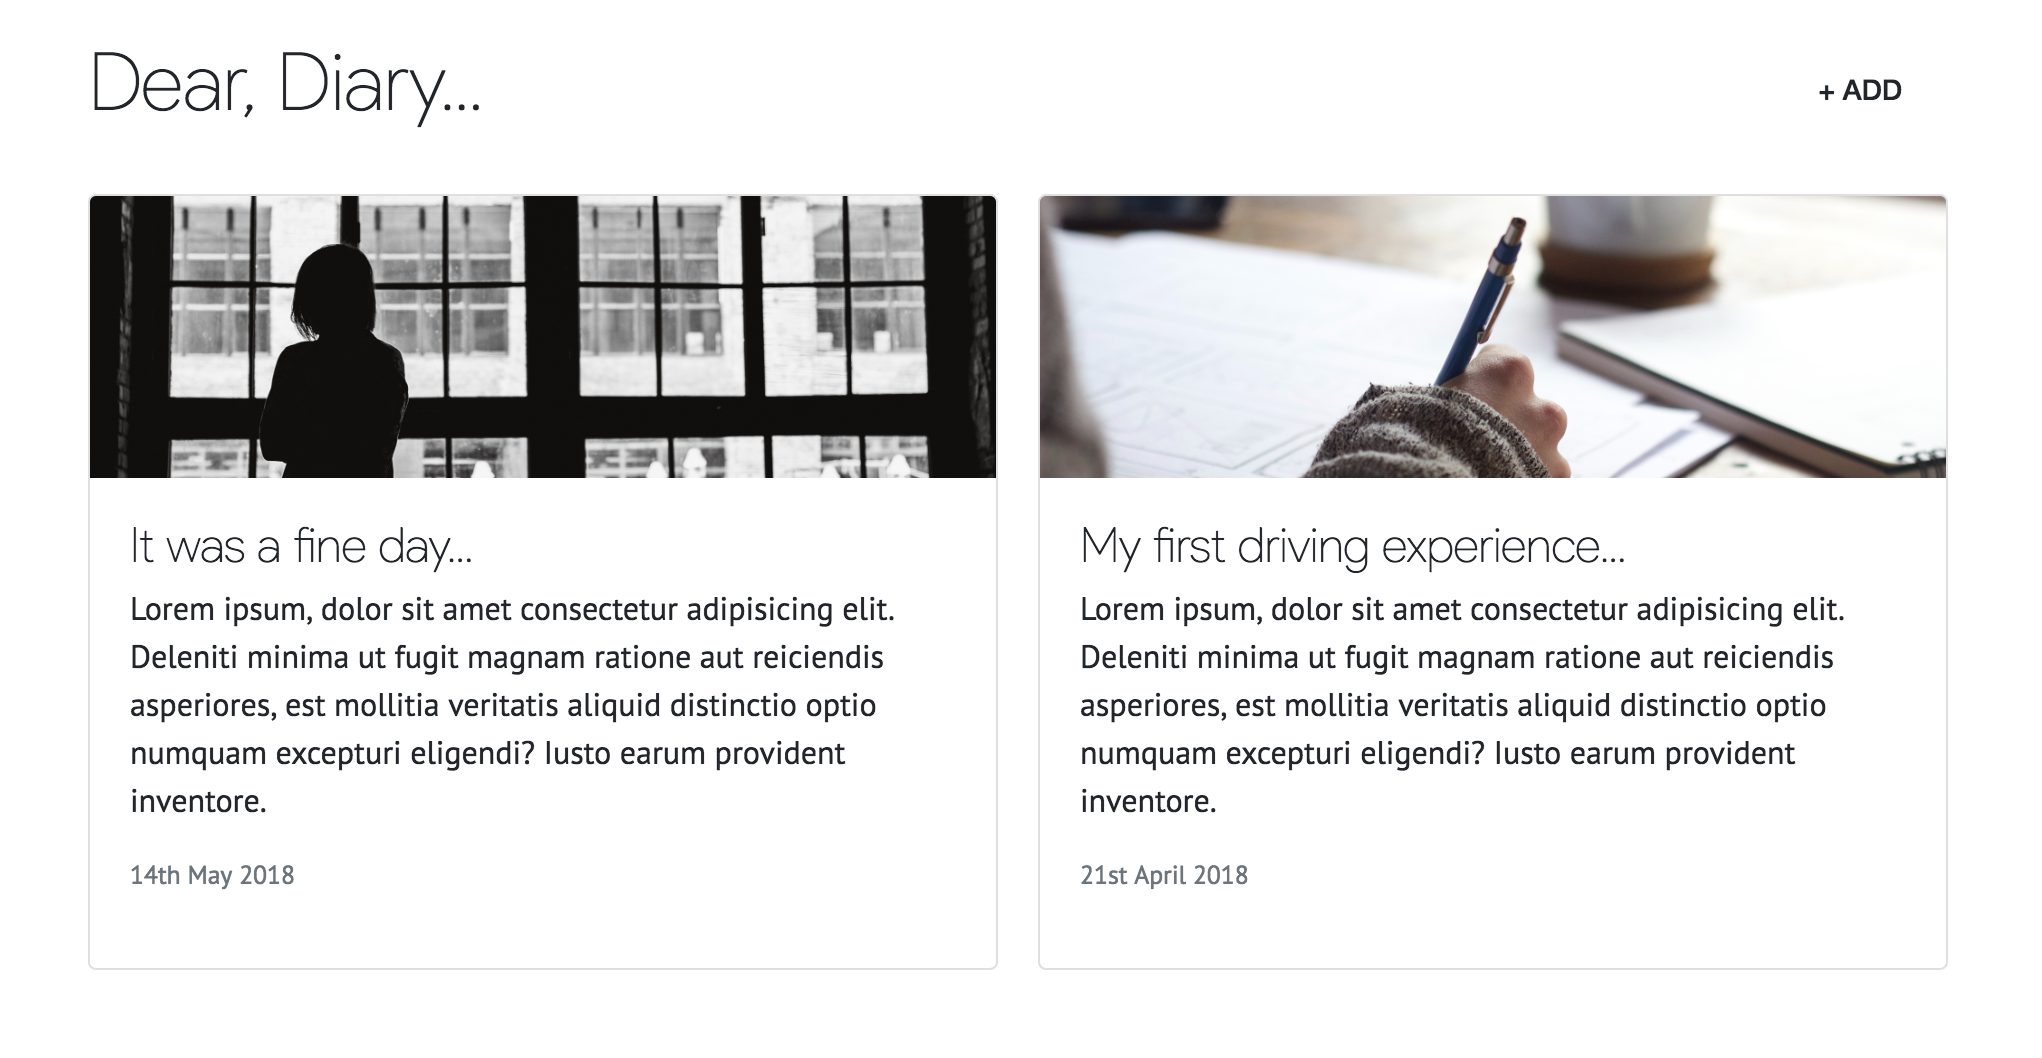
\includegraphics[width=\textwidth]{images/screenshots/website/website-dear-diary.png}
    \caption{Module \#1 - Dear Diary}
\end{figure}
\vspace*{\fill}

\pagebreak

\vspace*{\fill}
\begin{figure}[H]
    \centering
    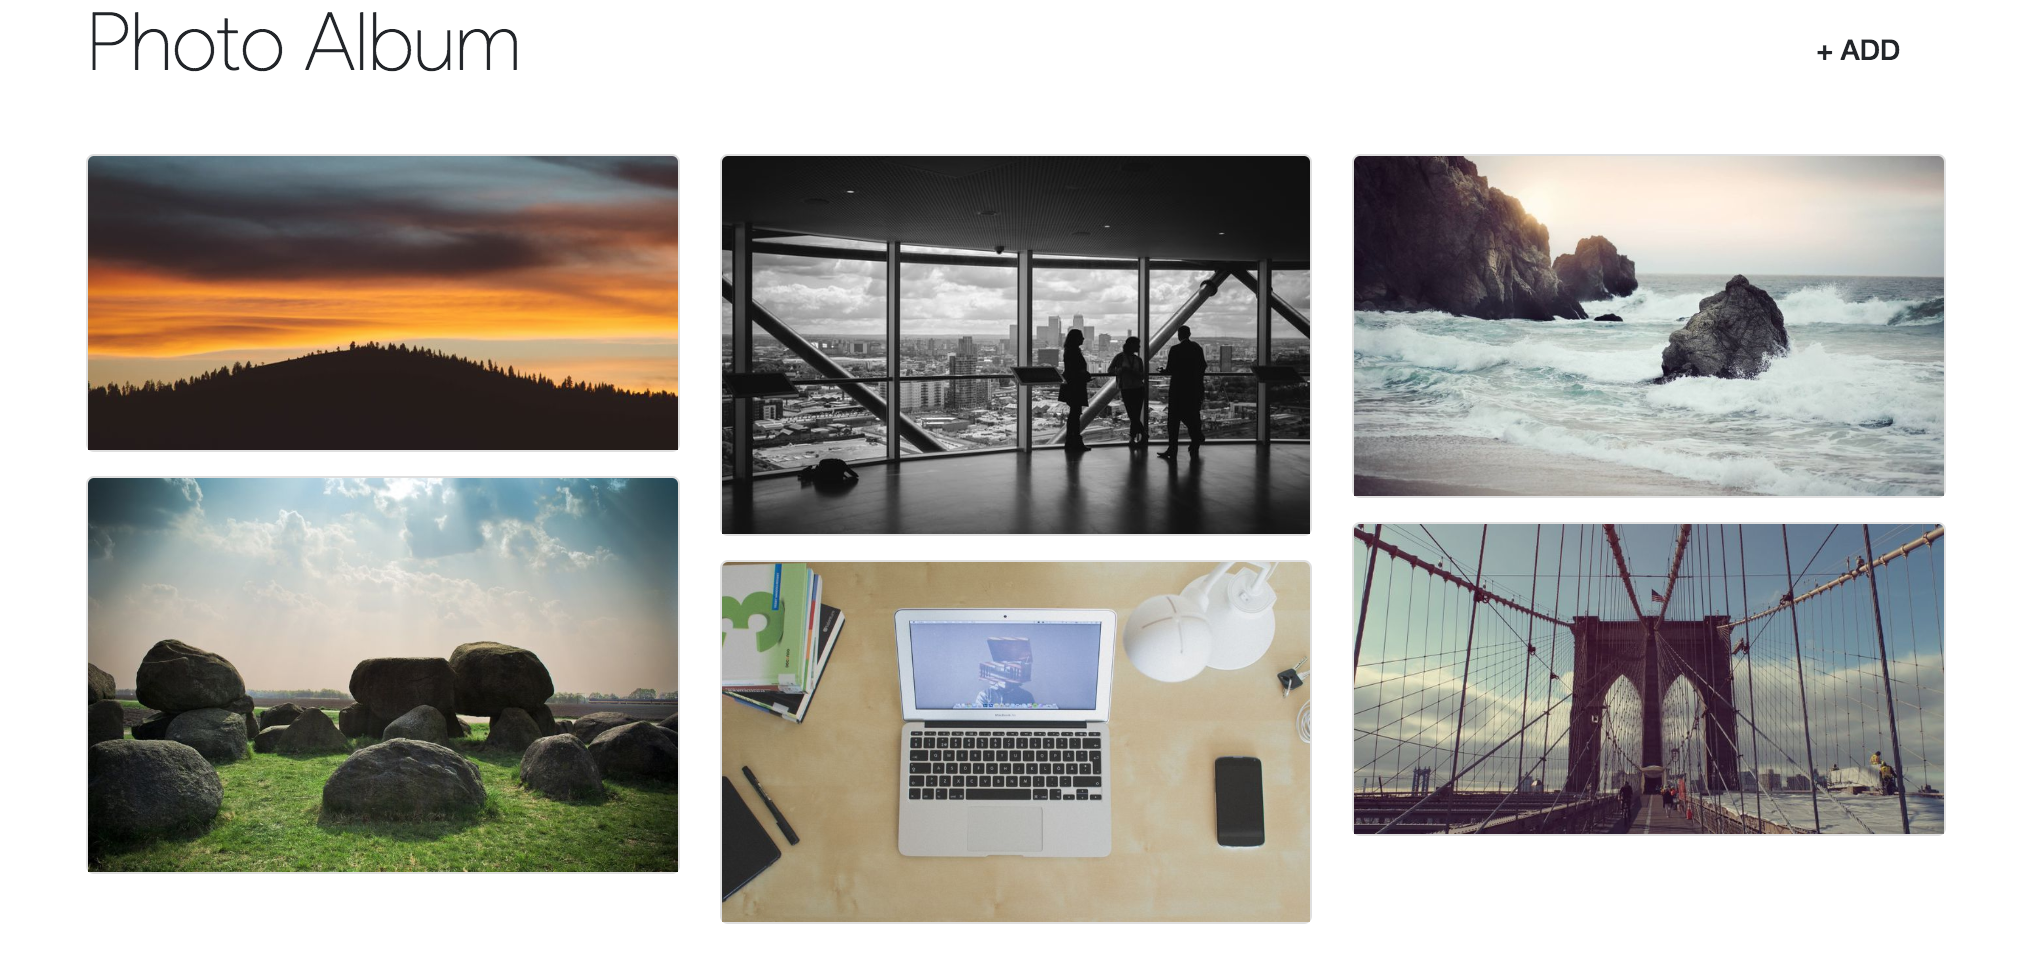
\includegraphics[width=\textwidth]{images/screenshots/website/website-photo-album.png}
    \caption{Module \#2 - Photo Album}
\end{figure}

\begin{figure}[H]
    \centering
    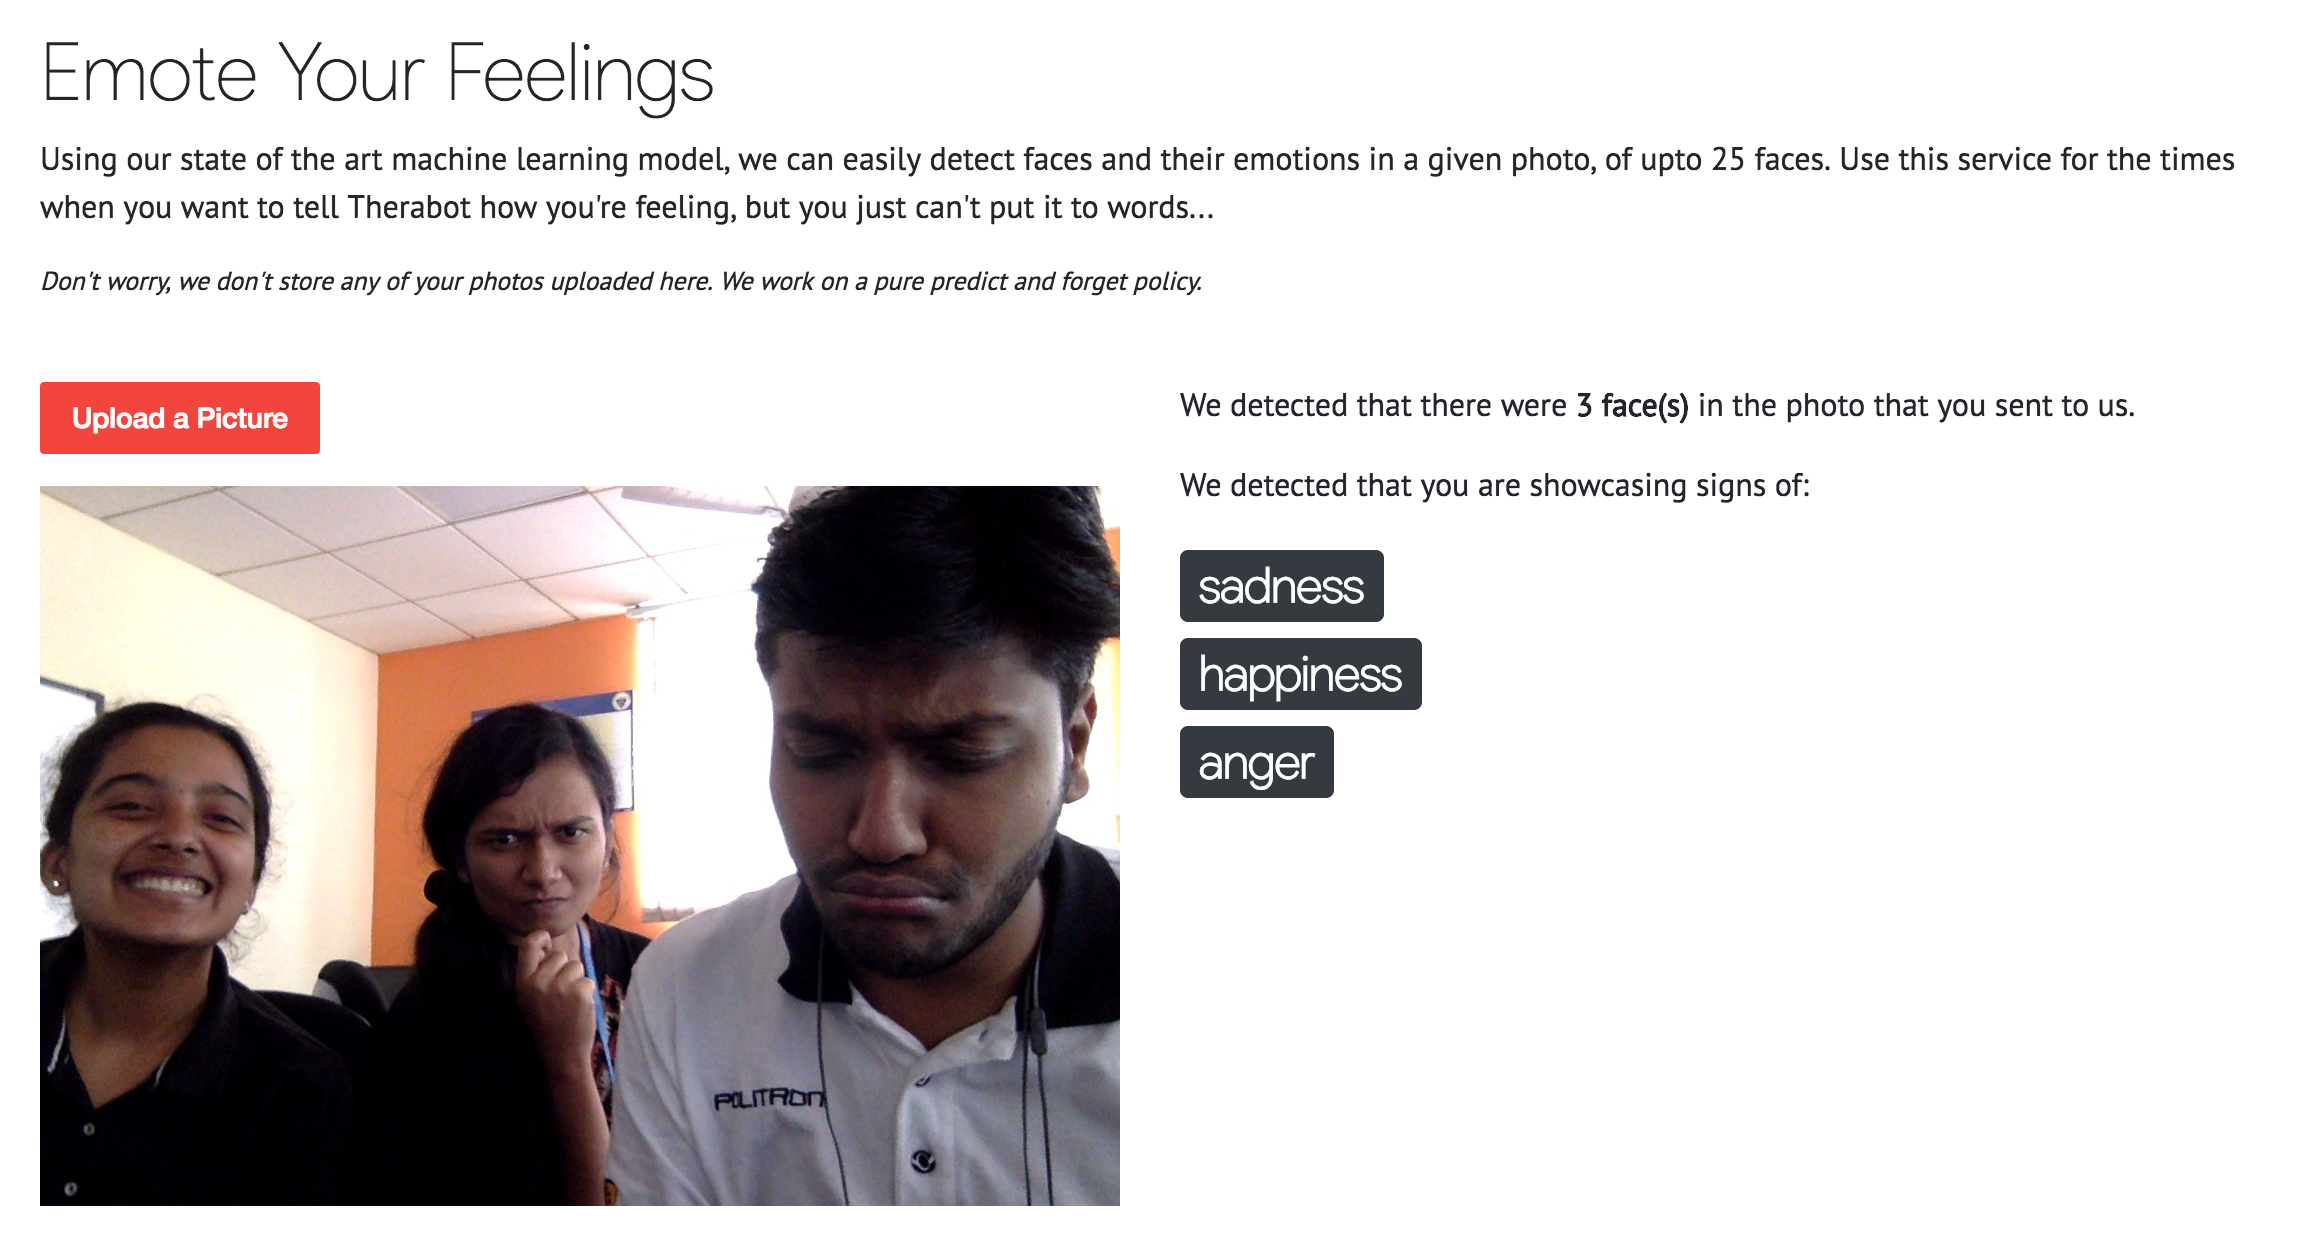
\includegraphics[width=\textwidth]{images/screenshots/website/website-emote-feelings.png}
    \caption{Module \#3 - Emote your Feelings}
\end{figure}
\vspace*{\fill}

\pagebreak

\subsection{Chatbot}

\noindent
Below are some screenshots of the chatbot, and it’s various conversational trees showcased in action:

\vspace*{\fill}
\begin{figure}[H]
    \centering
    \begin{minipage}{0.45\textwidth}
        \centering
        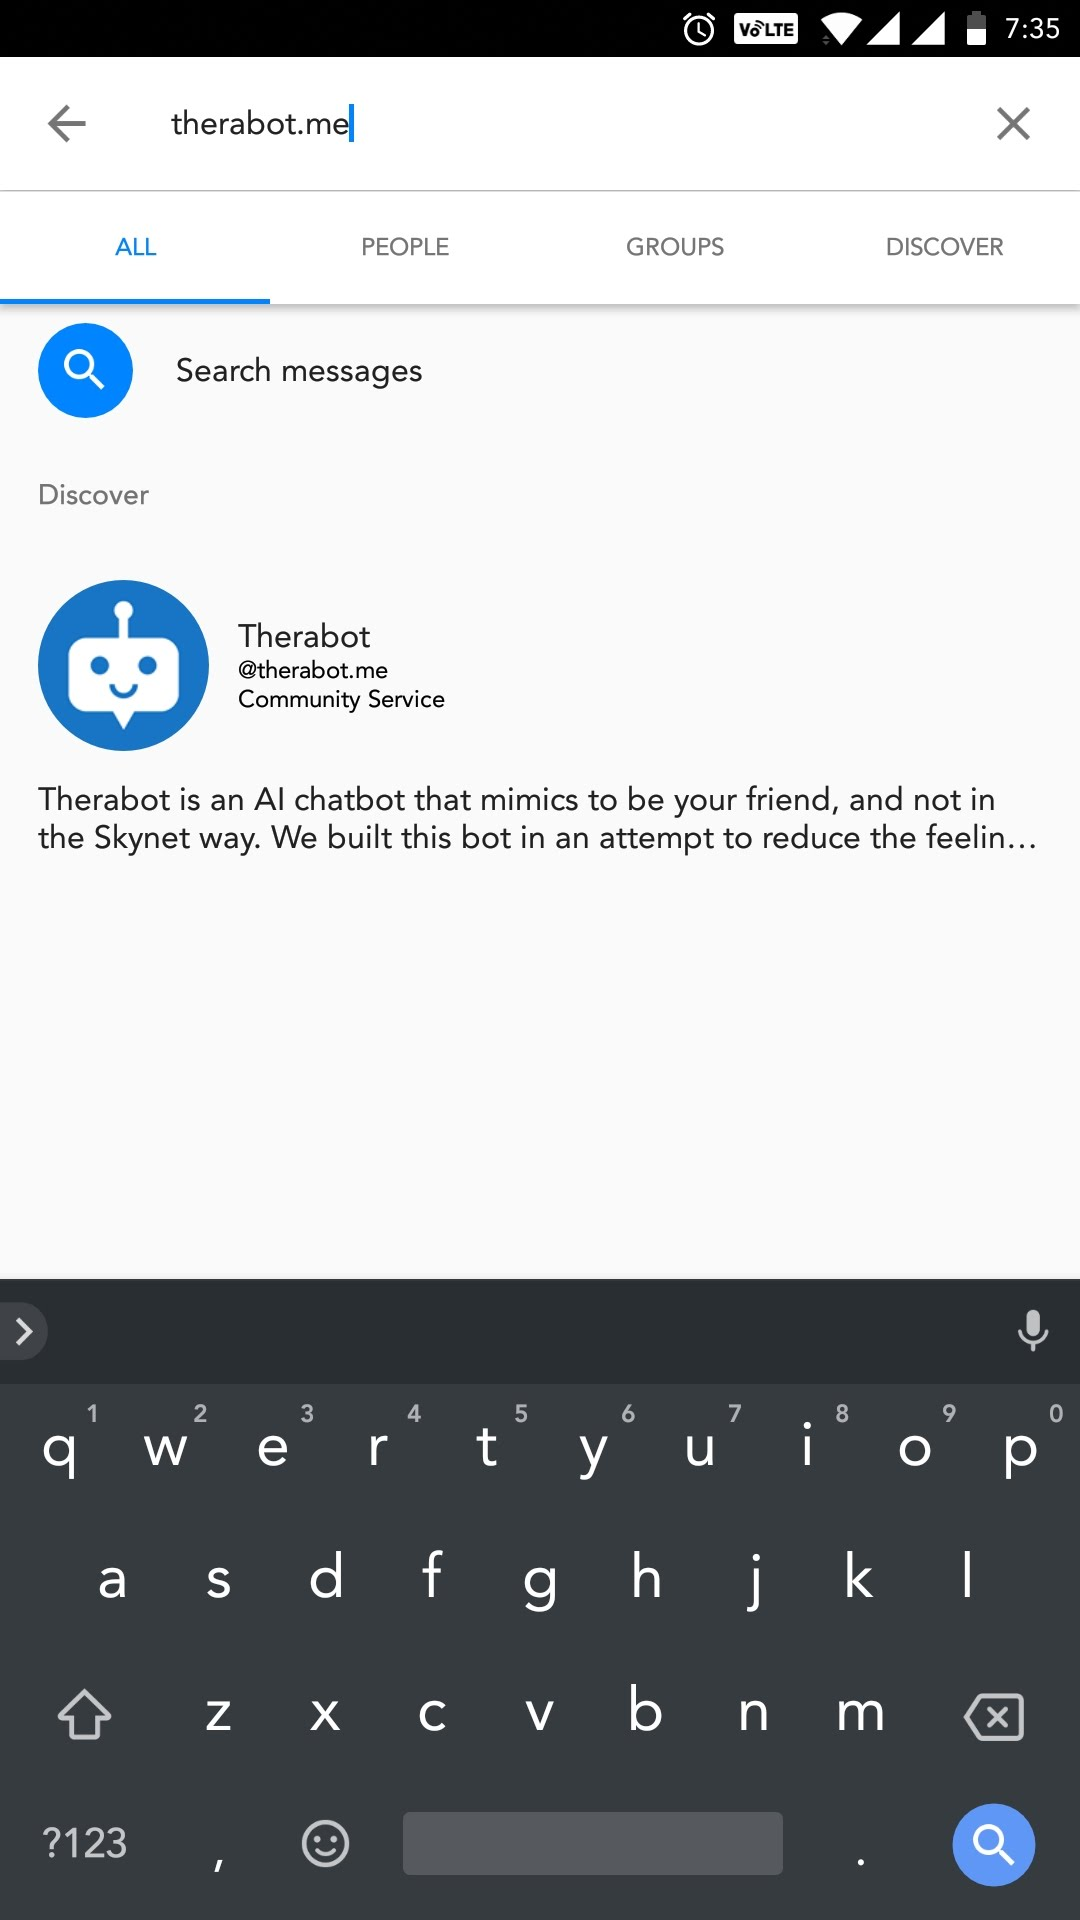
\includegraphics[width=0.9\textwidth]{images/screenshots/chatbot/1.jpg}
        \caption{Facebook Messenger}
    \end{minipage}\hfill
    \begin{minipage}{0.45\textwidth}
        \centering
        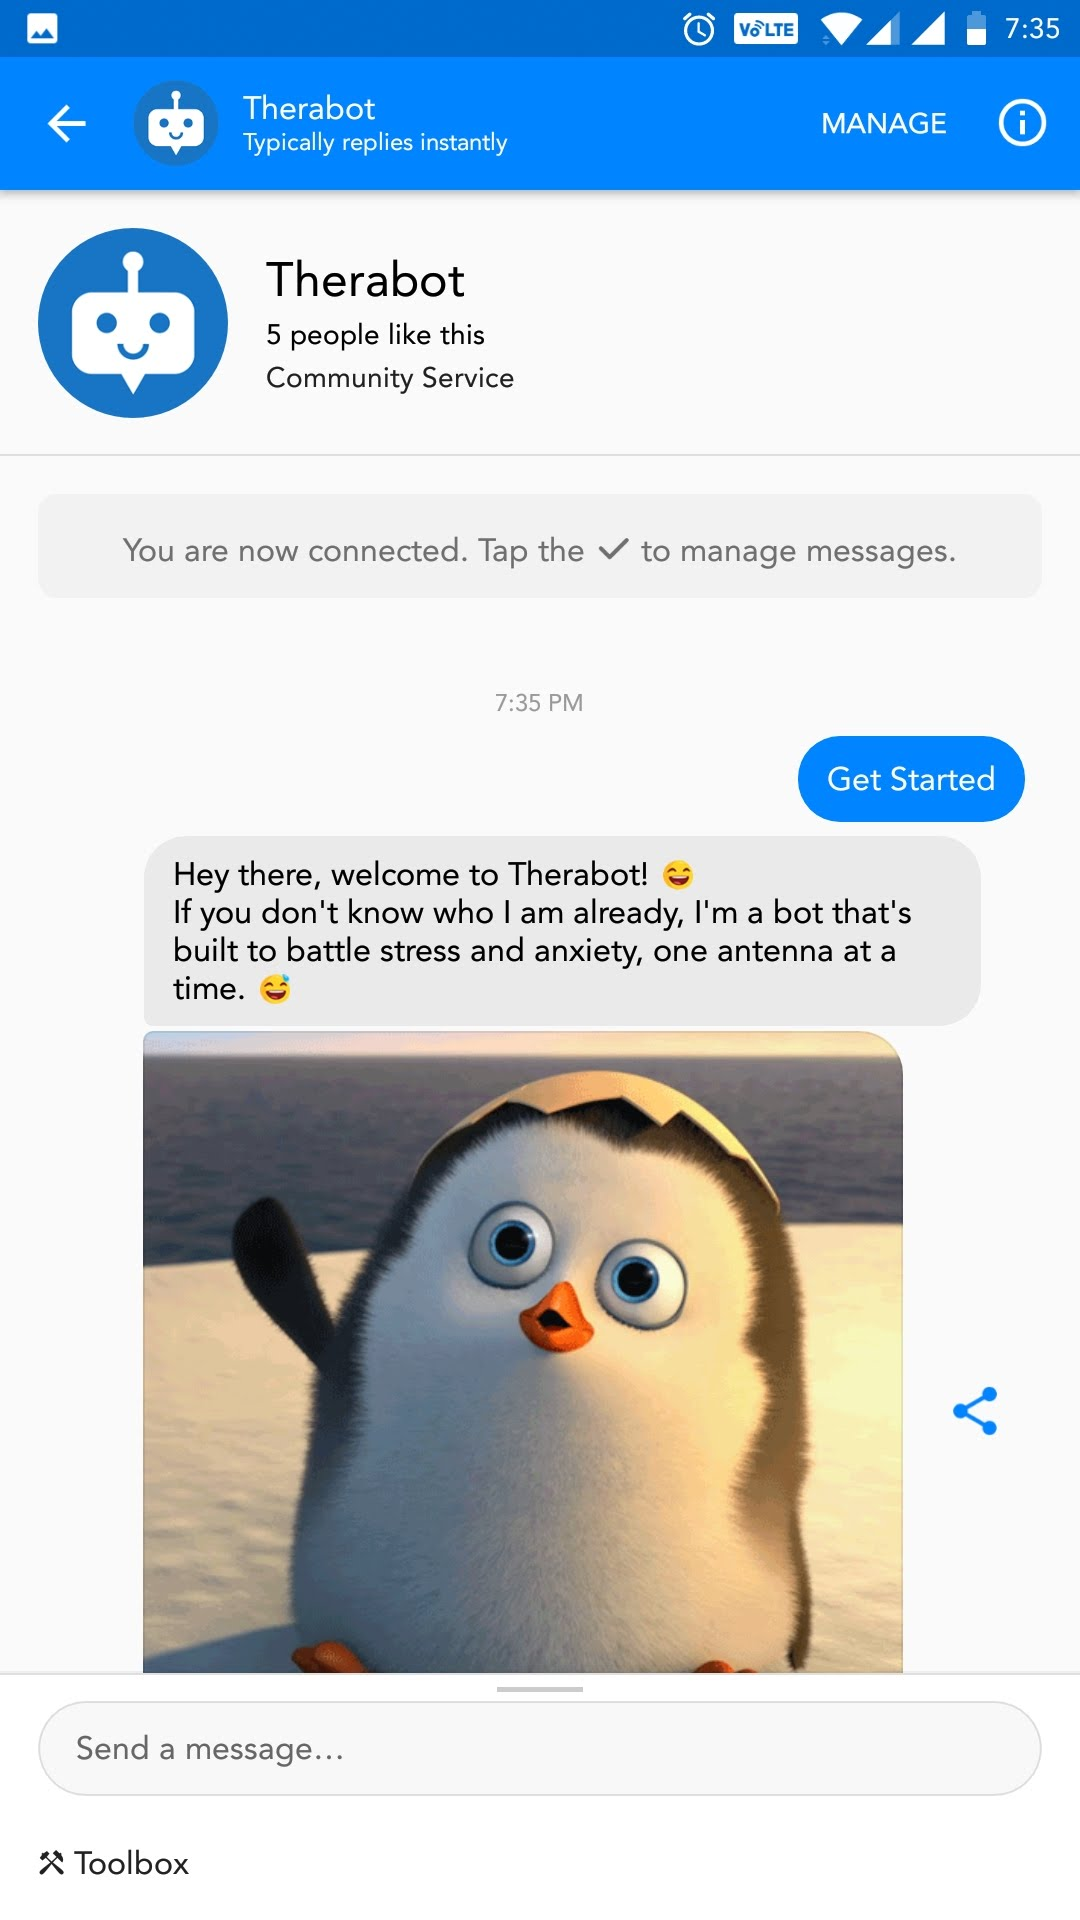
\includegraphics[width=0.9\textwidth]{images/screenshots/chatbot/2.jpg}
        \caption{User Onboarding}
    \end{minipage}
\end{figure}
\vspace*{\fill}

\pagebreak

\vspace*{\fill}
\begin{figure}[H]
    \centering
    \begin{minipage}{0.45\textwidth}
        \centering
        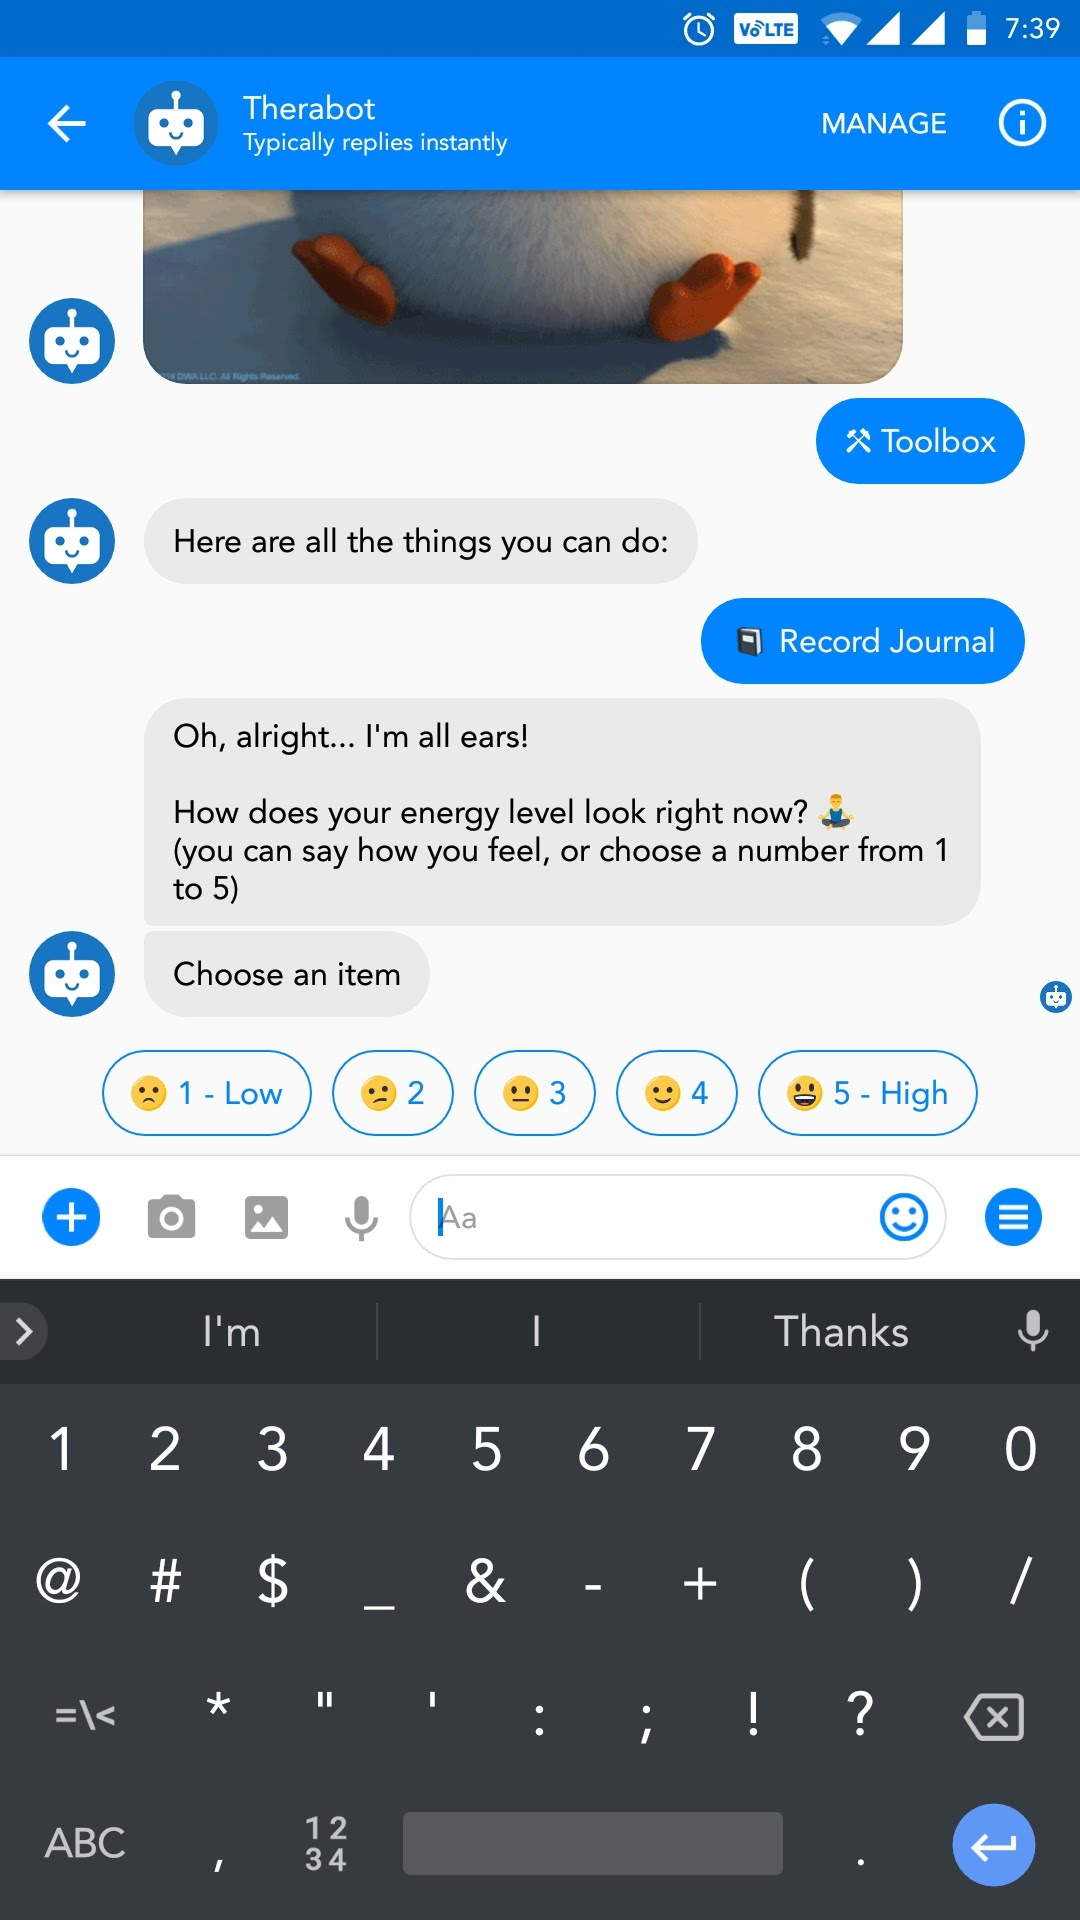
\includegraphics[width=0.9\textwidth]{images/screenshots/chatbot/3.jpg}
        \caption{Record Journal}
    \end{minipage}\hfill
    \begin{minipage}{0.45\textwidth}
        \centering
        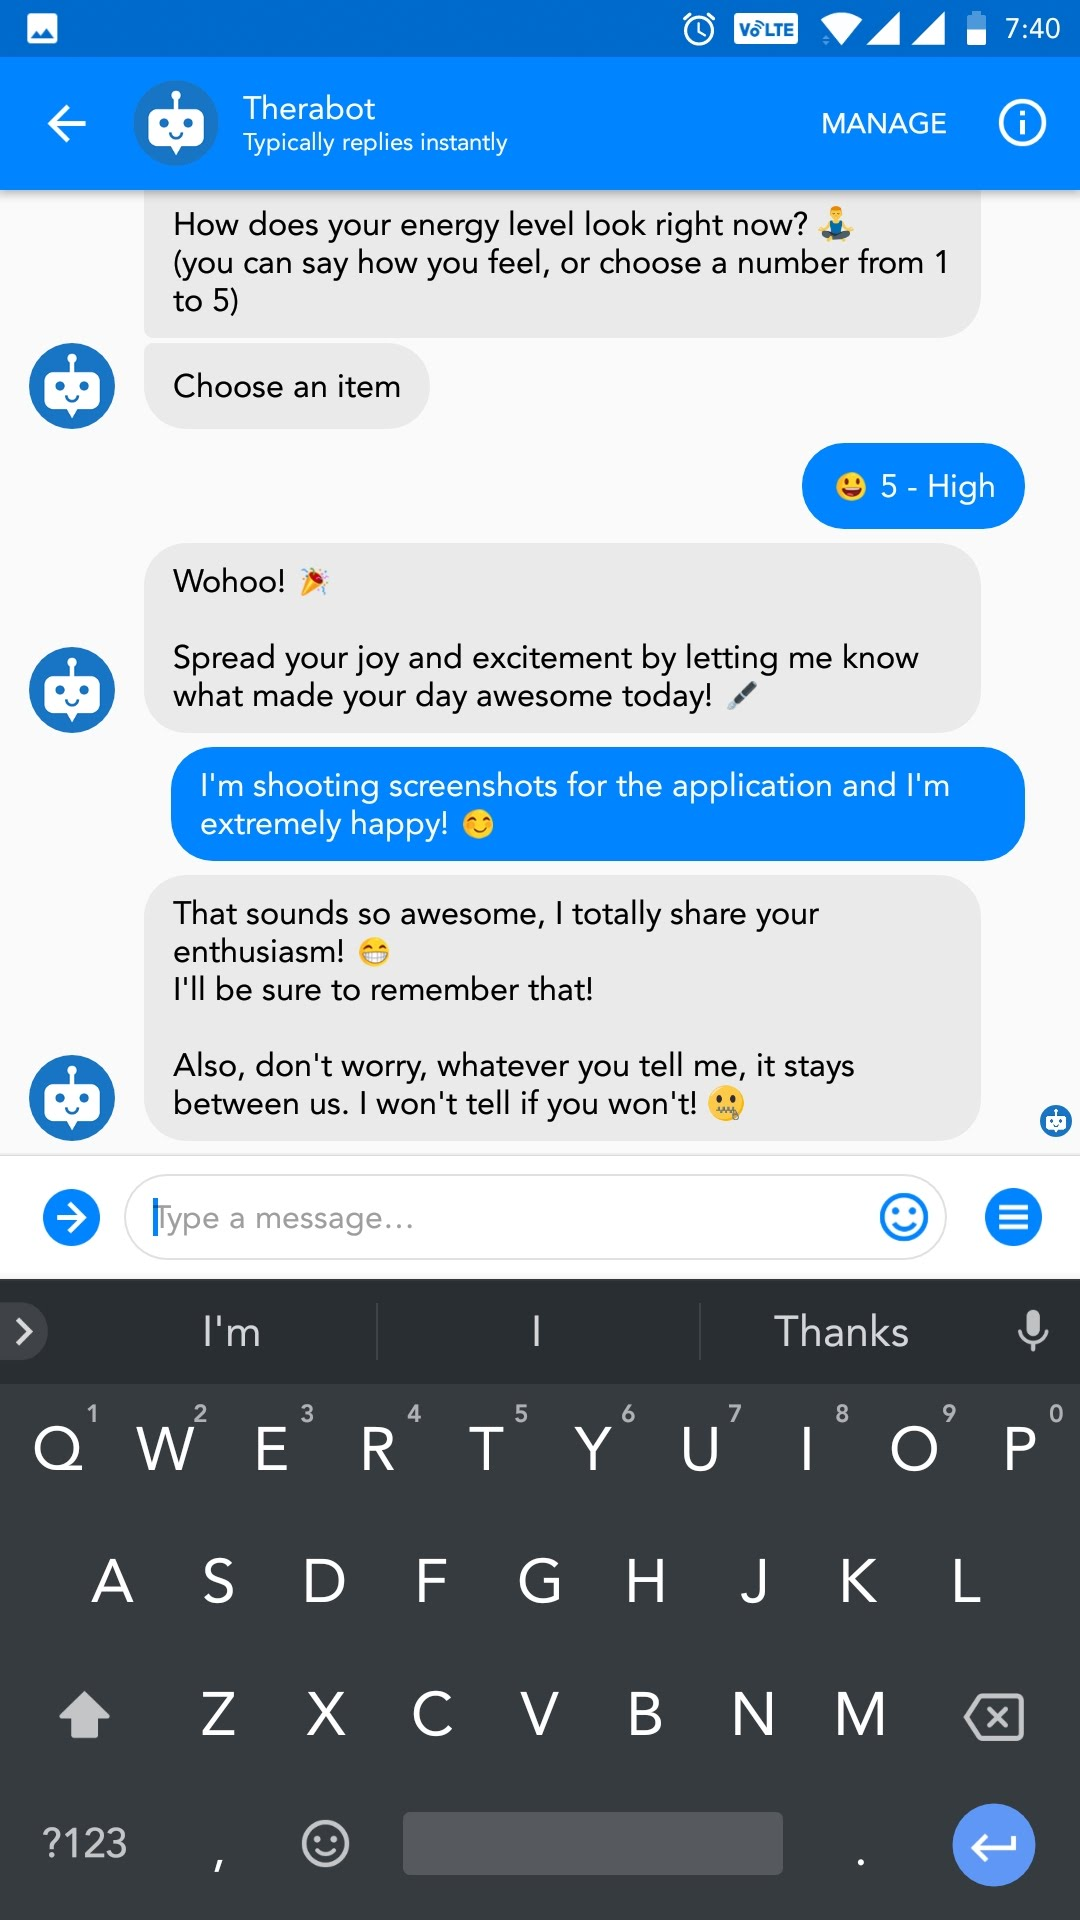
\includegraphics[width=0.9\textwidth]{images/screenshots/chatbot/4.jpg}
        \caption{Saving Journal Entry}
    \end{minipage}
\end{figure}
\vspace*{\fill}

\pagebreak

\vspace*{\fill}
\begin{figure}[H]
    \centering
    \begin{minipage}{0.45\textwidth}
        \centering
        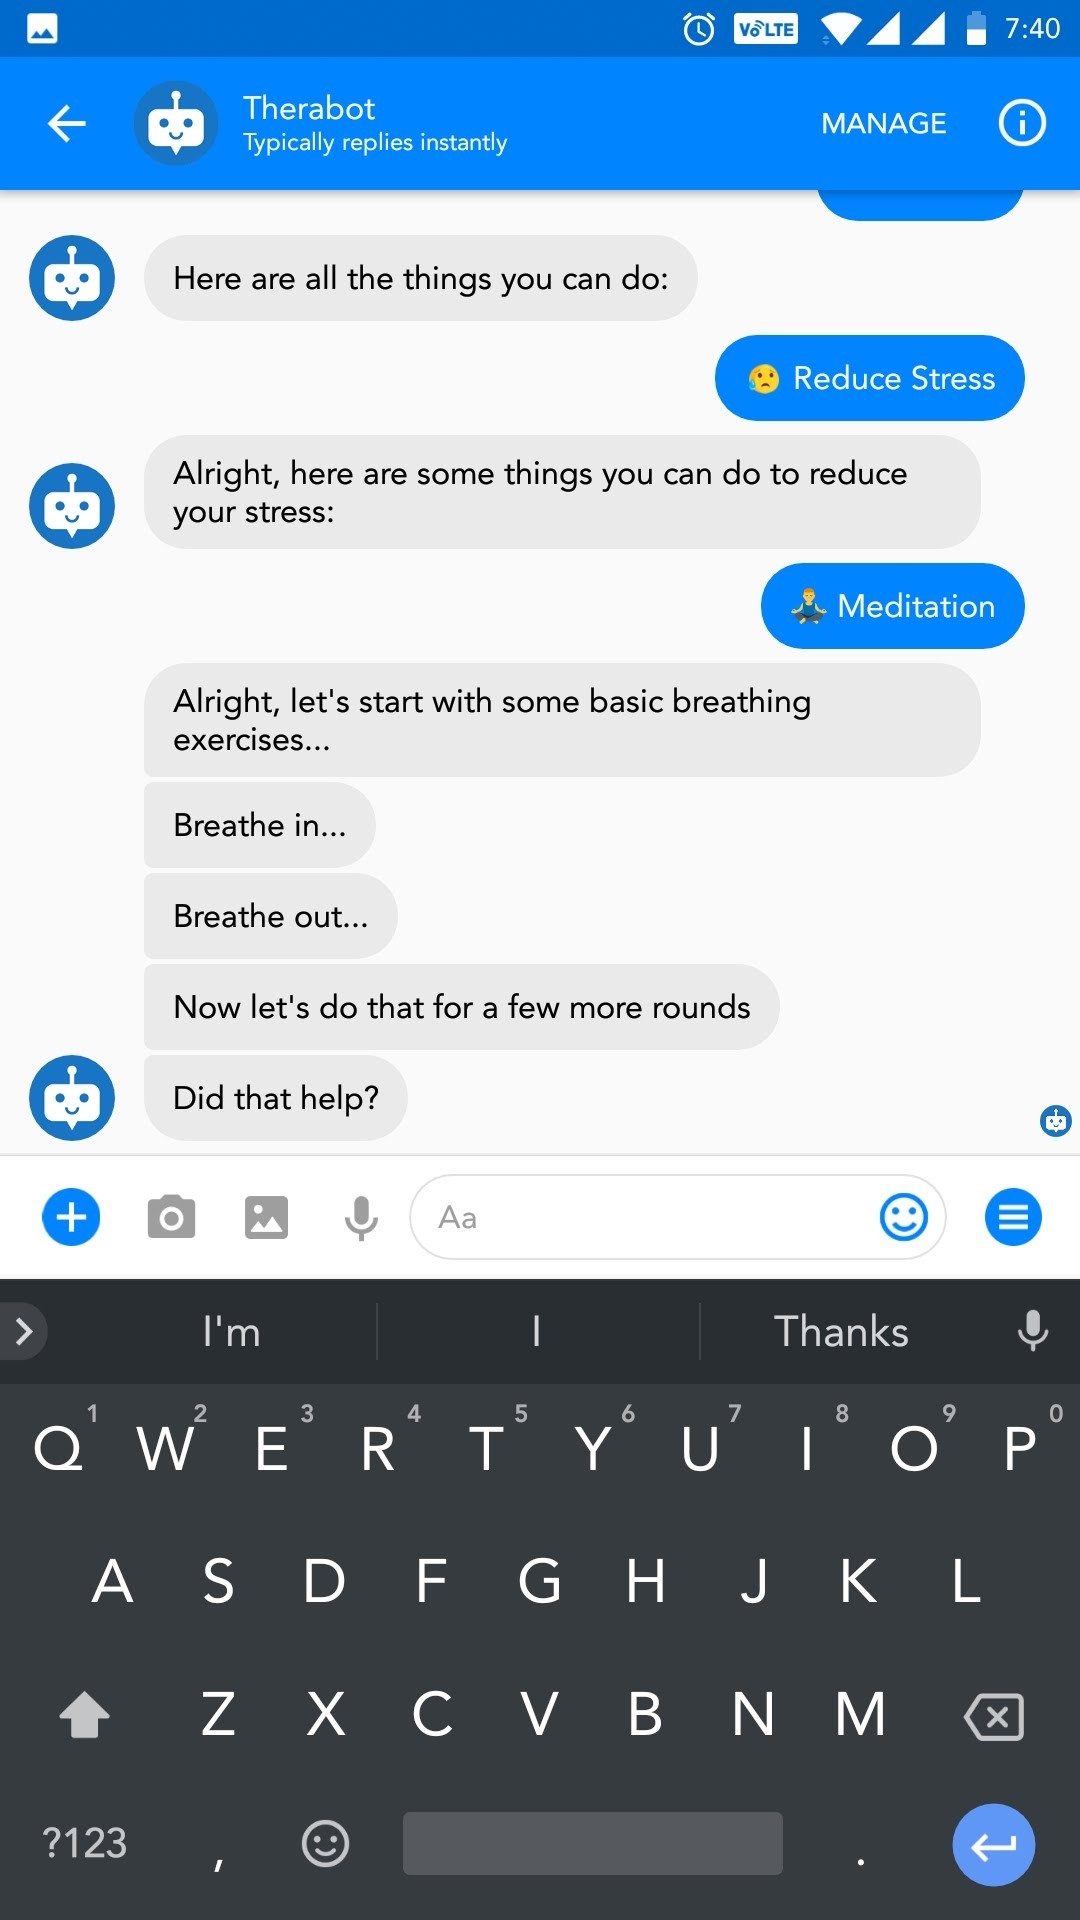
\includegraphics[width=0.9\textwidth]{images/screenshots/chatbot/5.jpg}
        \caption{Meditation}
    \end{minipage}\hfill
    \begin{minipage}{0.45\textwidth}
        \centering
        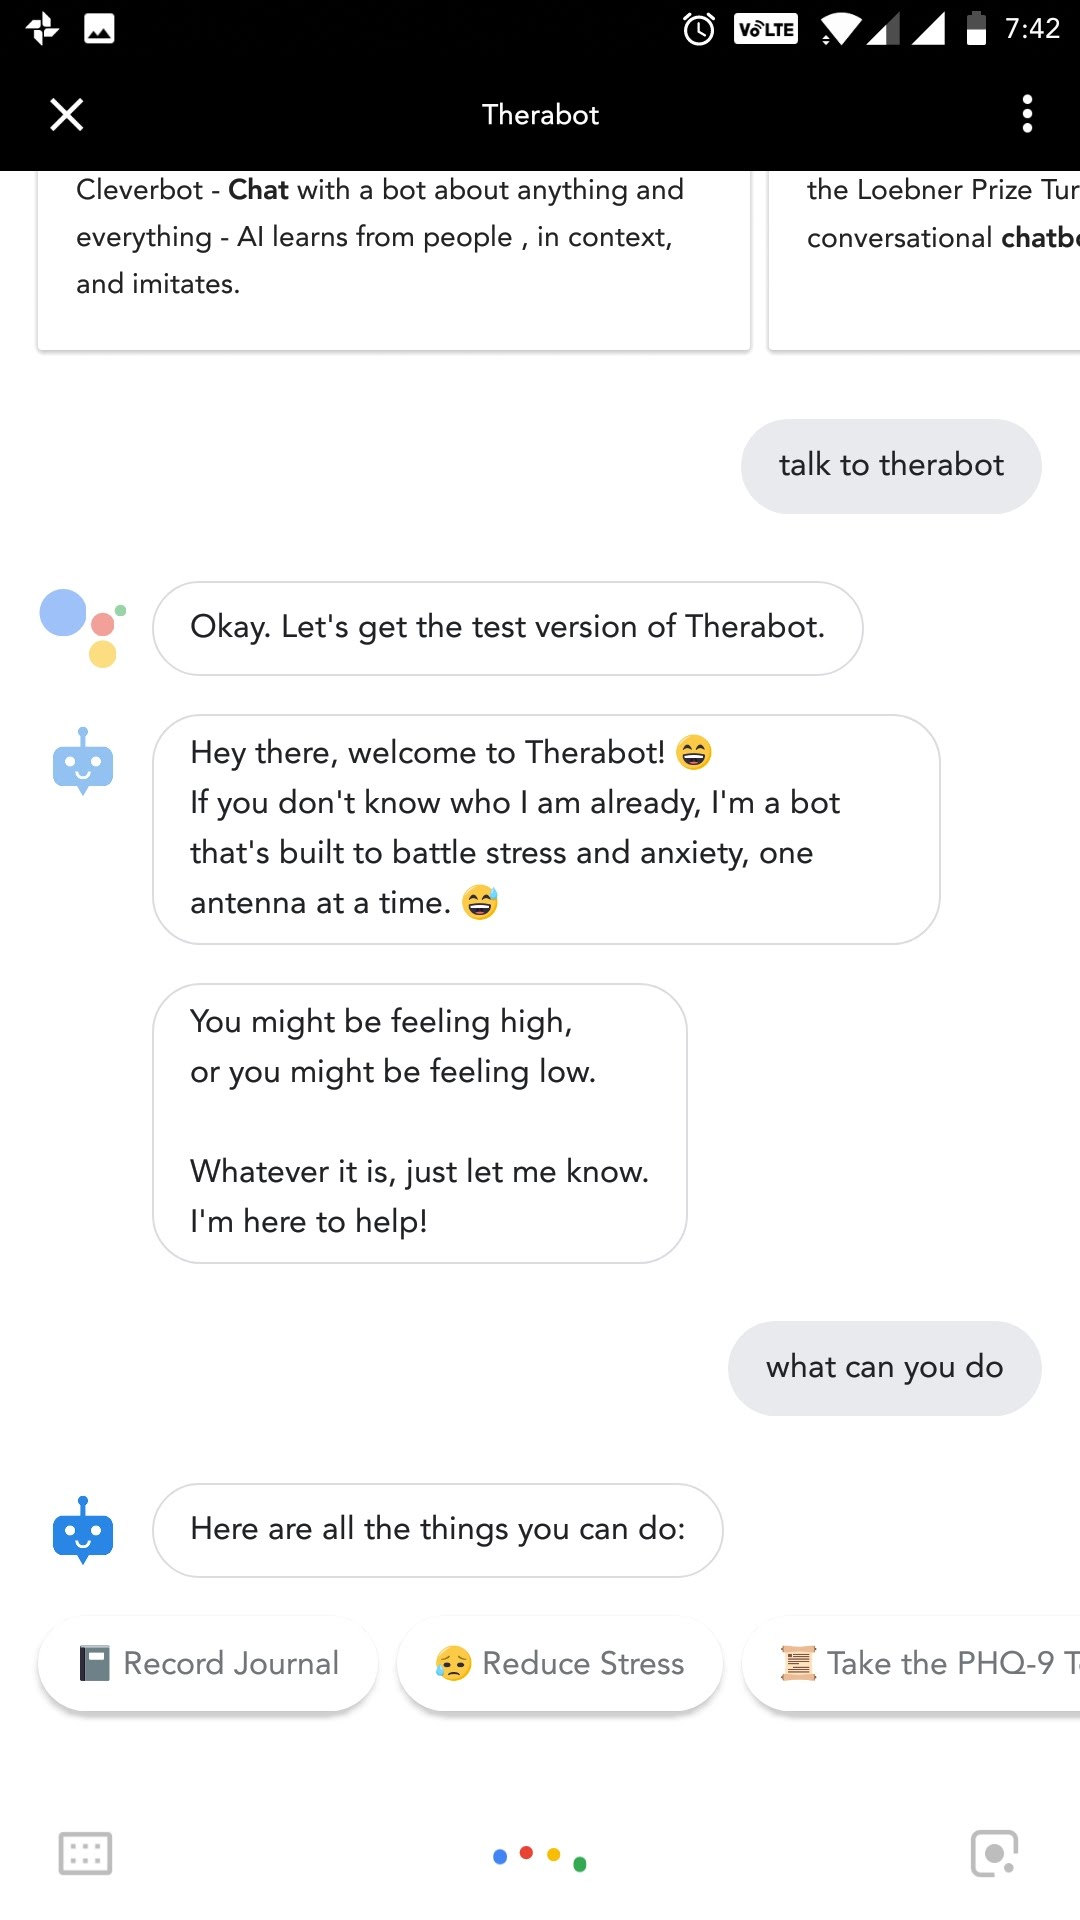
\includegraphics[width=0.9\textwidth]{images/screenshots/chatbot/6.jpg}
        \caption{Google Assistant}
    \end{minipage}
\end{figure}
\vspace*{\fill}

\pagebreak

\vspace*{\fill}
\begin{figure}[H]
    \centering
    \begin{minipage}{0.45\textwidth}
        \centering
        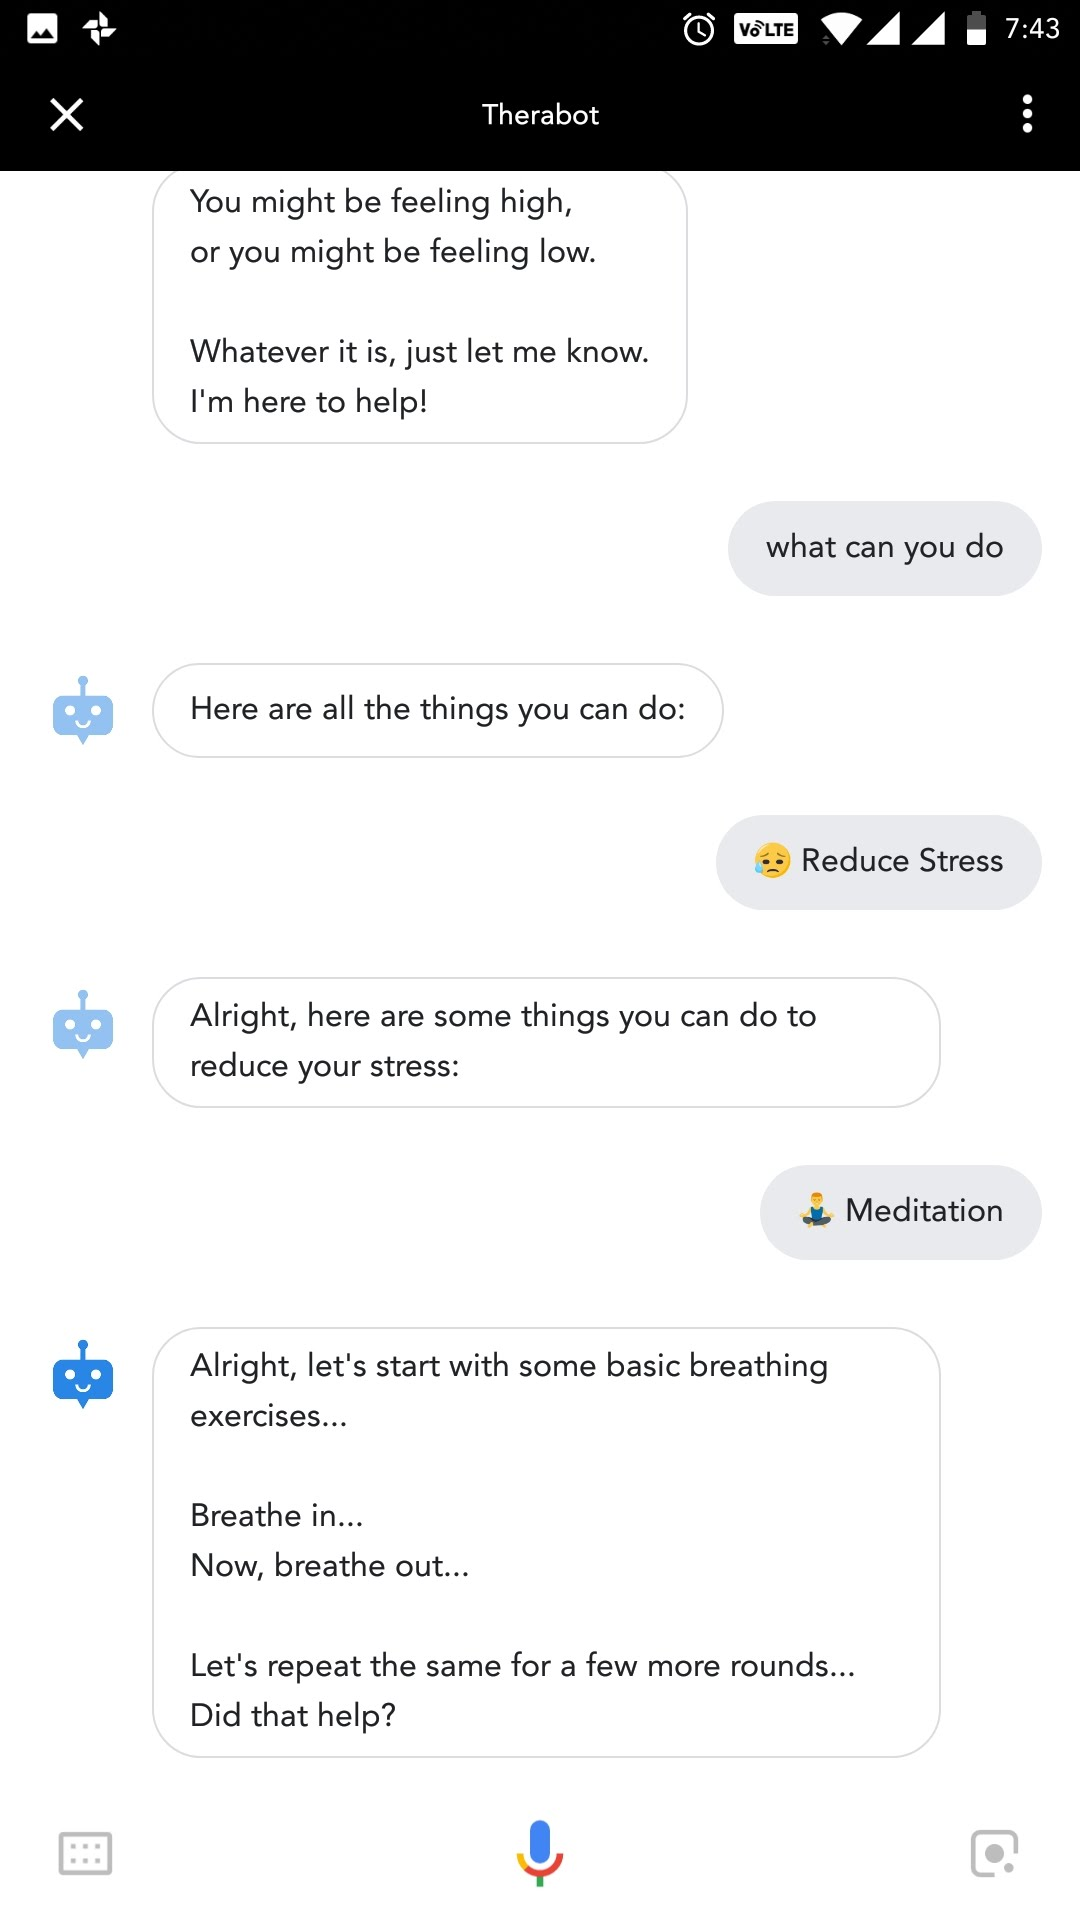
\includegraphics[width=0.9\textwidth]{images/screenshots/chatbot/7.jpg}
        \caption{Meditation w/ SSML}
    \end{minipage}\hfill
    \begin{minipage}{0.45\textwidth}
        \centering
        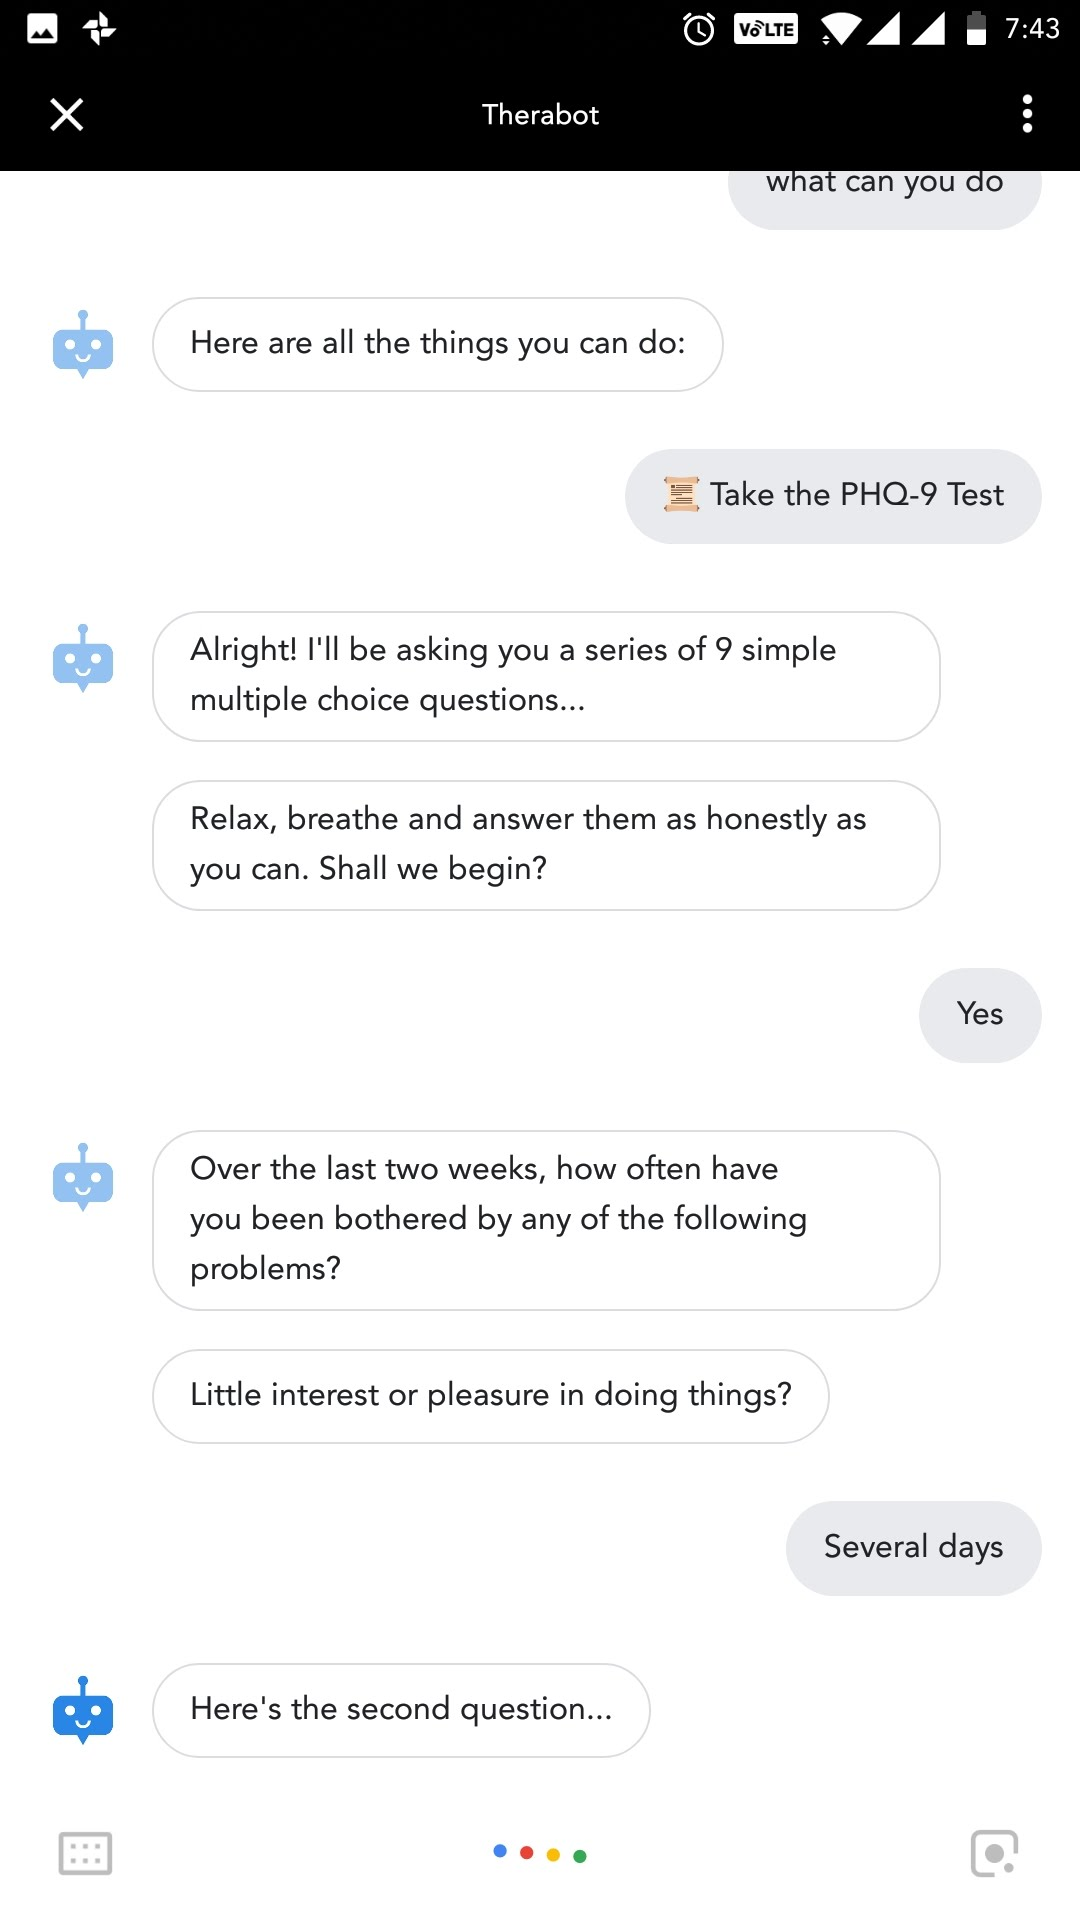
\includegraphics[width=0.9\textwidth]{images/screenshots/chatbot/8.jpg}
        \caption{PHQ9 Test}
    \end{minipage}
\end{figure}
\vspace*{\fill}

\pagebreak

\vspace*{\fill}
\begin{figure}[H]
    \centering
    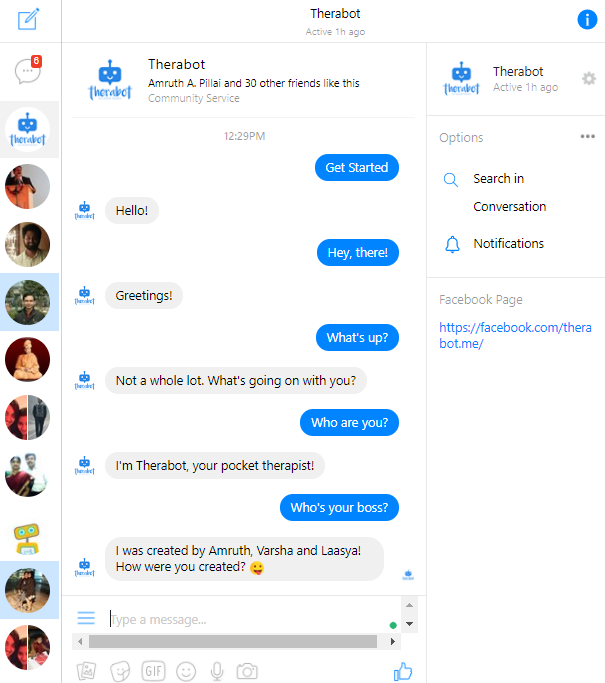
\includegraphics[width=12cm]{images/screenshots/chatbot/tablet.png}
    \caption{Tablet Screenshot}
\end{figure}

\begin{figure}[H]
    \centering
    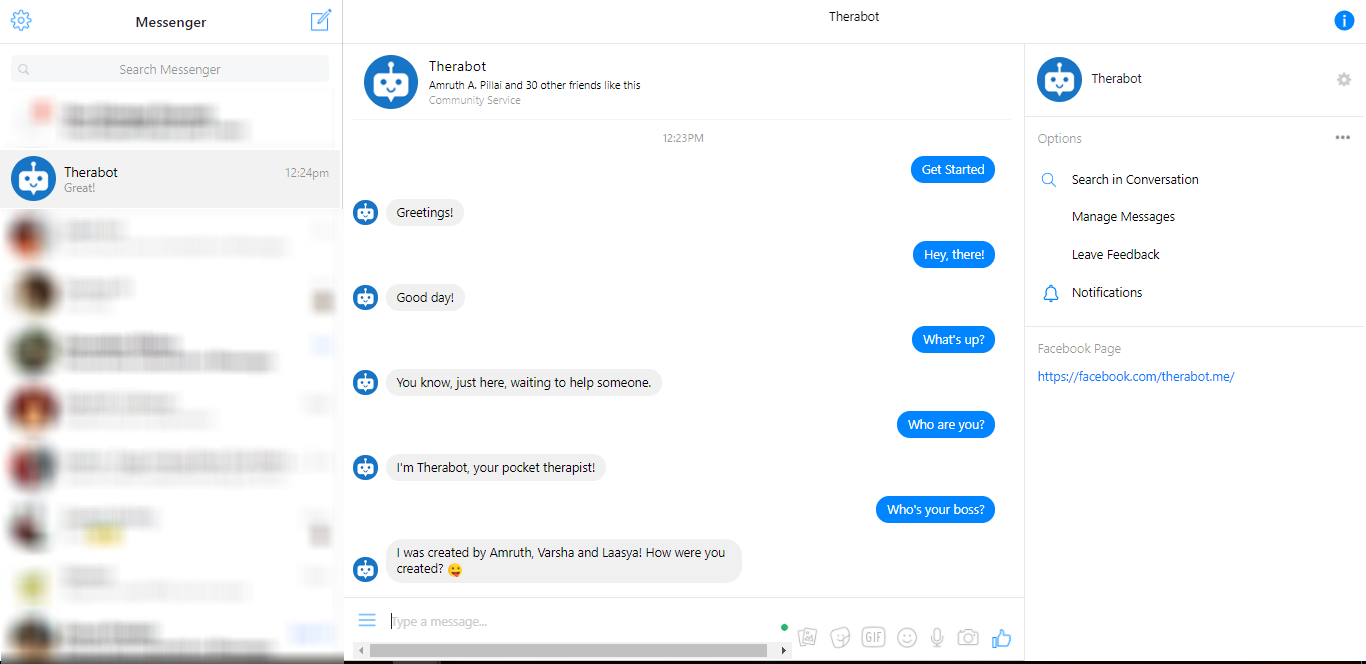
\includegraphics[width=\textwidth]{images/screenshots/chatbot/desktop.png}
    \caption{Desktop Screenshot}
\end{figure}
\vspace*{\fill}